\chapter[A Preliminary understanding of the global terrorism database]{Data understanding of the GTD}
\chaptermark{Data understanding of GTD}
\label{sec:appendixprelim}

\section{Introduction to terrorism incident databases}
As part of a larger initiative to apply machine learning techniques to the study of terrorism a initial data understanding was taken as part of the data mining process.  CRISP-DM \citep{chapman2000crisp} was used which consists of six phases, these are:

\begin{enumerate}
\item Business understanding. This introductory step of the analysis is aimed at getting an understanding of the purpose of the project and resulting requisites from a business point of view and transforming these into data mining problem statement. 
In the context of this project, the data mining problem statement would be to investigate if the application of data mining techniques to the study of terrorism is appropriate. Through the use of on-line terrorist incident  databases, to determine if its possible to determine changes in intensity or behaviour using machine learning. Particularly this is the application of machine learning techniques to investigate underlying spatial, temporal, regional and attack vector type relationships or associations. With the aim of gaining an understanding of the data and the methodologies that are most appropriate to the analysis of the data. Specifically, to see what insights can be gained from these methodologies, particularly the discovery of unusual time series count events. A number of count time series analysis techniques were investigated so as to determine their usefulness in modelling terrorist incident data. 
\item Data understanding. This stage begins with a commencing assessment of the data involving a compiling of the data necessary to carry out the analysis after which a number of activities are carried out to gain a familiarity with the data and to establish if data quality issues exist within the data. Secondly to determine initial insights or to find compelling sub-populations within the data on which to construct a number of hypothesis on veiled or obfuscated information which may exist within the data. In the context of this investigation the data is provided by the GTD. The data quality problems associated with the dataset are highlighted in section~\ref{sec:markermeasdif}. However due to collection process and data encoding process (detailed in the GTD codebook) employed by the GTD, the data understanding was a relatively easy task.
\item Data preparation. This stage would traditionally deal with assembly of the full final dataset, however as the data was already pre-assembled this stage was not required. Instead various aggregation operations utilizing R's data aggregation capabilities were carried out.  
\item Model building. During this stage a number of different modelling techniques are applied. To make the data applicable to the specific data mining techniques, a number of data preparation tasks may be required. Therefore an iterative approach, returning back to the data preparation step was required. In the context of this analysis this involved both joining the GTD to other datasets or aggregating or sub-setting the data. While in the context of modelling or visualizing time series data experimenting with different time intervals would be a typical task undertaken in the analysis. This was achieved by aggregating the data at different time intervals (week, day, month, year).
\item Model evaluation. During this step the model construction and any insights gained from the model are evaluated. Data modelling was carried out in two stages firstly an initial exploratory modelling phase was carried which evaluated some preliminary modelling techniques. After evaluation of the preliminary modelling techniques additional modelling techniques were evaluated which overcame specific deficiencies in the preliminary techniques. Model evaluation was carried out in a number of ways:
\begin{itemize}
 \item Checking model specification, this involves the determination of the suitability of a modelling technique to a particular task by determining if the correct iid (independently and identically distributed variables) have been included and if the model meets any underlying assumptions of the modelling technique.
 \item Checking the accuracy of the model. This involves  a determination of the accuracy of a particular modelling technique. This is a specially difficult task for unsupervised techniques.
 \end{itemize} 
\item Model Deployment. During this step the model is deployed in a production setting, however this stage is not applicable in the current setting. Though consideration should be given to techniques which are more generalizable as these would be easier to deploy and use. 
\end{enumerate}

\section{Data mining techniques used in the preliminary understanding of the GTD database data}

Preliminary analysis was used to gain an initial understanding of the GTD through the use of a number of geo-spatial, regio-specific and regio-temporal patterns this was done using a mix of descriptive visualization. Dimension reduction and preliminary modelling were also used to gain an understanding of the GTD but also to see which modelling techniques might be applicable to its study. A broad range of different techniques were applied, these techniques included:
\begin{enumerate}
\item Data visualization. A number of data visualization techniques were used to gain an initial understanding of evolution of terrorism from a temporal, attack vector type and regional perspective. Unsupervised techniques, both hierarchical and K-Means clustering, were utilized to gain a better understanding of spatio temporal terrorist patterns (particularly regio-specific attack types). These techniques were used in conjunction with both static and interactive visualization to enhance and ease analysis, particularly with the spatio clustering of terrorist incidents using leaflet \citep{leaflet2016}. To accomplish this, interactive spatial visualization in conjunction with clustering is used to show the concentration of terrorist incidents in urban areas. 

This section can be seen as a an extension of descriptive analytics using visualizations. Descriptive analytics can be seen as the most basic form of analytics as they allow alot of data to be condensed into smaller more effective and insightful packets of information. The purpose of the descriptive analytics is to provide more purposeful and useful information in a more digestible form. The descriptive analytics are then visualized using an appropriate visualization technique or provided in tabular format. 

Dimension reduction along with visualization offers a level of analysis over more traditional descriptive analytics and can be seen as providing a level of reduction in complexity of data and offering more insightful information. Dimension reduction allows higher dimension data to be summarized in fewer dimensions while maintaining the variation of the original data in these new dimensions.  Both the creation of summary statistics and simple data visualization and dimension reduction can be seen as a form of descriptive analytics. Both forms of descriptive analytics allow the analyst to uncover underlying patterns within the data.

\item Dimension reduction techniques. Dimension reduction techniques (in the context of this project this can be considered an unsupervised learning technique as opposed to a data pre-processing step) are used to gain a better understanding of the interaction between multiple data dimensions. With the use of data visualization techniques and the descriptive statistics used as described above, they are limited to analysis of a small number of dimensions (three to four dimensions). Dimension reduction techniques used in conjunction with interactive data visualization techniques allow the researcher to gain a better insight into the data by allowing the ability to analyse multiple dimensions with many levels and drill deep into the data. This would not be possible with static data visualizations of the data as the visualizations would become crowded and difficult to understand. In this section/appendix correspondence (CA) and multiple correspondence analysis (MCA) \citep{factominer2008} are utilised to carry out dimension reduction on a number of categorical dimensions (CA and MCA can be seen as analogous to principal component analysis but for categorical data) and the results are then visualized using Plotly \citep{plotlymanual2016}. 
\item A number of preliminary modelling techniques are to used to gain a further understanding of the temporal spatial and attack vector types. A number of supervised methods particularly count regression techniques and Hidden Markov Models (HMM's) for the analysis of time series data of deaths due to terrorism.  
\end{enumerate}

\section{Data mining techniques used in the preliminary understanding of the GTD database data}
\label{sec:chap4dataprep}

A number of different visualization techniques were used to explore the temporal and spatio temporal relationships between deaths due to terrorism.  These ranged from simple time series plots to stacked bar charts to various types of choropleths or thematic maps. Stacked bar plots were of particular use as they allowed the visual encoding of a third data dimension along with year and deaths due to terrorist incidents including region attack vector and weapon type. The static plots were created with ggplot2 \citep{ggplotwickham2009}, Hadley Wickham's own implementation of the grammar of graphics \citep{wilkinson2006grammar}. Dplyr \citep{dplyr2016wickham}, reshape2 \citep{reshape2007wickham} and tidyr \citep{tidyr2916Wickham} were used to manipulate and transform the data before visualizing the data. Typical transformations used are aggregation of data and conforming data to the correct shape through wide to long or vice-versa transformations.

Googlevis (which is an R wrapper around google's visualization library), Plotly \citep{plotlymanual2016} and leaflet \citep{leaflet2016} were used to create a number of interactive plots. Using leaflet and Googlevis to create interactive choropleths offers a number of advantages over traditional static methods as more information can be stored through the use of interactive layers and captions which can display further information in call out boxes. This allows further number of data dimensions to be visually encoded allowing more subtle understanding of the data.

\subsection{The evolution of terrorism over time (year and month) by
region and world wide}\label{sec:evteryearmonth}

Plotting the monthly totals of deaths due to terrorism by regional and by world wide figures,  using these two plots , temporal and regio-temporal relationships emerging. The relationships are shown in figures \ref{fig:tseriesmonth1} and \ref{fig:tseriesmonthregion1}and can be summarized as:

\begin{enumerate}
\item
  Since records have started to be recorded in 1970, deaths due to terrorism are on the rise. From the time series world plot we see that during the 1980's there was a sharp rise in terrorism. This flattened out with end of the cold war and appears to be declining up to the end of 1990's, while after September the 11th 2001 there is an increase in  terrorism. This increases dramatically with the invasions of Iraq and  Afghanistan, it steadily increases upto 2007, before sharply rising after 2010, specifically after the rise of ISIS in Syria and Iraq after 2012.
\item
  When examining the time series plot by month and by region, a more  refined pattern is clear. A spike in terrorism can be seen in the 1980's due to a sharp rise in terrorism in Central America and later in the decade in South America. This fell at the end of the 1980's and start of the 1990's. Terrorism fell across all regions before beginning to rise in the 2000's especially in sub-Saharan Africa, the Middle East and North Africa and south Asia (particularly Afghanistan and Pakistan).
\end{enumerate}
The time series plot for the different regions is shown in figure~\ref{fig:tseriesmonthregion1}. The
temporal, regional relationships described above are clearly visible (see figure~\ref{fig:tseriesmonthregion1}).

\begin{figure}[t]
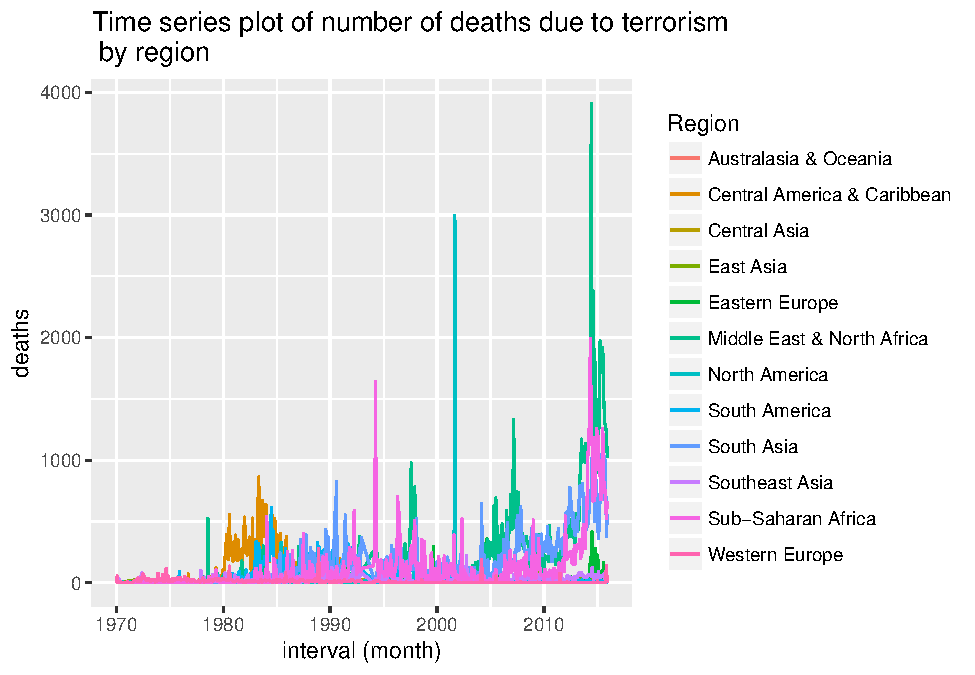
\includegraphics[width=10cm]{C:/Users/Peter/Desktop/Peters_experiment_markdown_files/figure-latex/unnamed-chunk-2-1.pdf}
\caption{Time series plot interval (month) of deaths by region}
\label{fig:tseriesmonthregion1}
\centering
\end{figure}

\subsection{The evolution of terrorism over time (month) by
region}

While the world wide time series plot (by time interval month) quite clearly shows the rise in terrorism worldwide since 1970 (see figure~\ref{fig:tseriesmonth1}). Plotting by region shows the specific temporal regional relationships are clearly visible, these are the sharp rise in the 1980's to the start of the 1990's of deaths due to terrorism in central and South America. Again a regional shift of deaths due to terrorism has shifted to the Middle East, this rose sharply after the September 11th attacks and the subsequent invasions of Afghanistan and Pakistan (see figure~\ref{fig:tseriesmonthregion1}).

\begin{figure}[t]
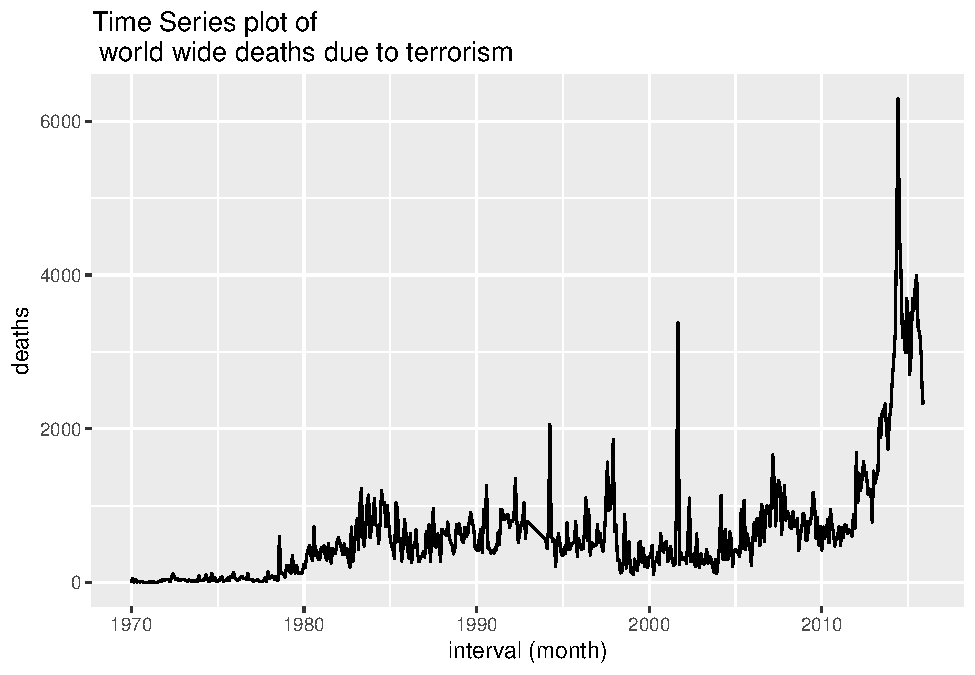
\includegraphics[width=10cm]{C:/Users/Peter/Desktop/Peters_experiment_markdown_files/figure-latex/unnamed-chunk-3-1.pdf}
\caption{Time series plot interval(month) of deaths}
\label{fig:tseriesmonth1}
\centering
\end{figure}

\subsection{The evolution of terrorism over time (year) by
region}

The rise in deaths to due to terrorism is more clearly observed (when using interval year) when the global rise in deaths due terrorism by year since 1970, using a year interval instead of month interval (which was used in the previous section~\ref{sec:evteryearmonth}). The pattern is even more clear when the time series of deaths by years and deaths by year and region is plotted. Figure~\ref{fig:tseriesyear1} shows the number of deaths globally (not broken out by region). A rise in the late 1970's and 1980's followed by a period of relative stabilization  which persisted till the early 2000's followed by a large increase thereafter is seen.

\begin{figure}[t]
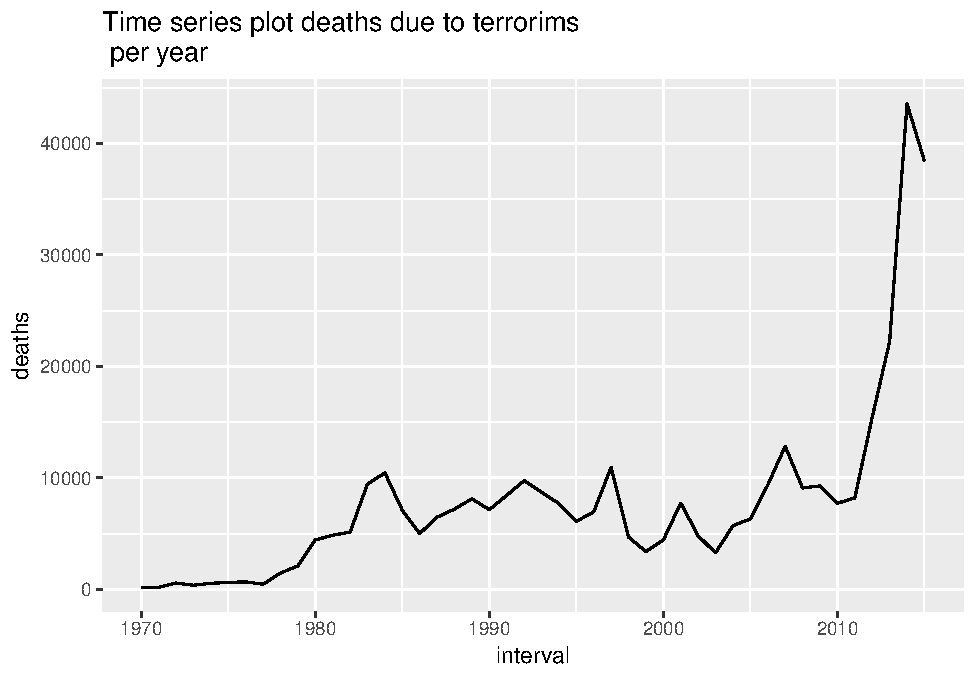
\includegraphics[width=10cm]{Peters_experiment_markdown_files/figure-latex/unnamed-chunk-4-1.pdf}
\caption{Time series plot interval(year) of deaths}
\label{fig:tseriesyear1}
\centering
\end{figure}

When viewing these deaths by  year and region. A clear pattern emerges the rise in number of deaths due to terrorism in Central America in the 1980's which fell
sharply towards the end of the cold war. A rise in terrorism is also clearly visible post the September the 11th attacks in North Africa and the Middle East and in South Asia, Figure~\ref{fig:tseriesyear2}.

\begin{figure}[t]
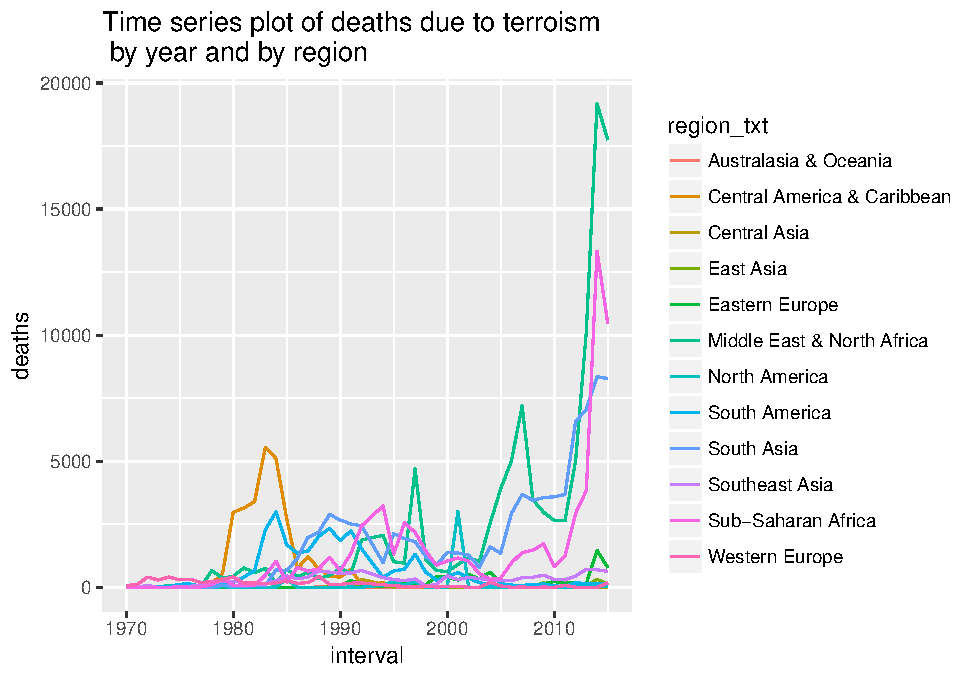
\includegraphics[width=10cm]{Peters_experiment_markdown_files/figure-latex/unnamed-chunk-5-1.pdf}
\caption{Time series plot interval(year) of deaths}
\label{fig:tseriesyear2}
\centering
\end{figure}

\subsection{The evolution of terrorism over time (year) by
region using stacked bar charts}

The regio-temporal shifts are even more evident when visualizing the data as a stacked bar chart, Figure~{fig:stackbaryear1}. The stacked bar chart allows the assessment of the contributing fraction of total deaths for a particular time interval by region. When viewed as a stacked bar plot (with the region represented as portion of the bar). It is clear to see the fall off in terrorism in South America and Central America (in the 1990's), corresponding with a rise in deaths due to terrorism in the Middle East and South Asia. For the last decade the number of deaths that are due to terrorism has been dominated by South Asia, the Middle East and Sub Saharan Africa. Note the gap at 1993 due to the loss of data from the GTD when transferring data from the Pinkerton agency to the GTD.

\begin{figure}[t]
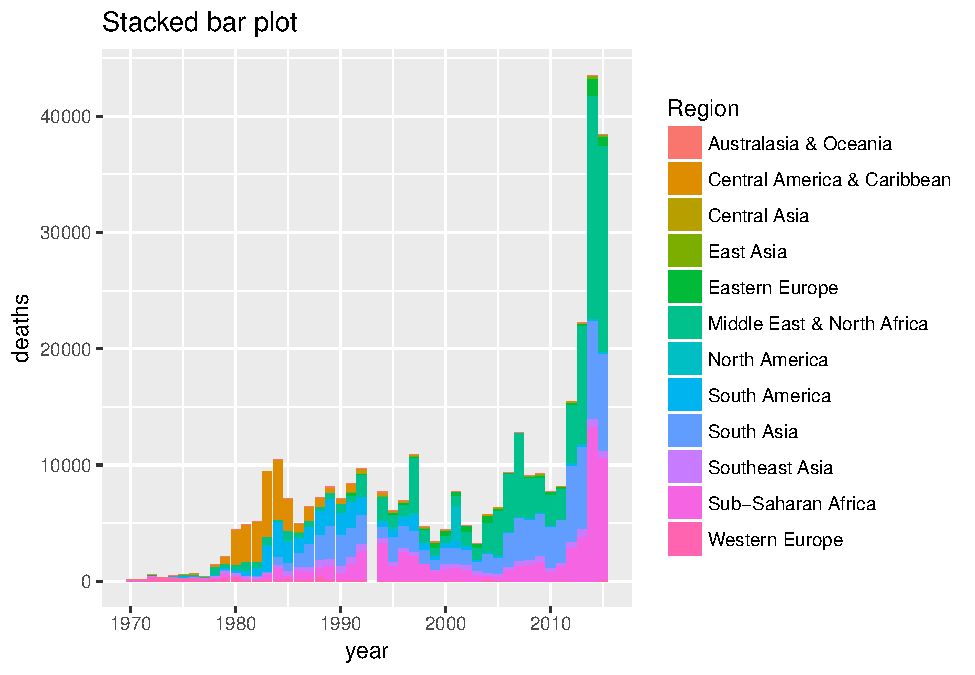
\includegraphics[width=10cm]{Peters_experiment_markdown_files/figure-latex/unnamed-chunk-6-1.pdf}
\caption{Stacked bar plot interval(year) of deaths}
\label{fig:stackbaryear1}
\centering
\end{figure}

\subsection{Visualizing deaths by attack vector and weapon type
type}\label{viewing-deaths-by-attack-vector-type}

Examining the plot of deaths due to attack vector (armed assault,
hijacking, hostage taking etc.) is shown in figure~\ref{fig:stackbaryearattackvector1}. Again a temporal relationship exists, since the 2000's emergence of bombings and explosives
as the prominent attack vector. Also the emergence of hostage taking
(barricade incidents and Kidnapping) is observed.

\begin{figure}[t]
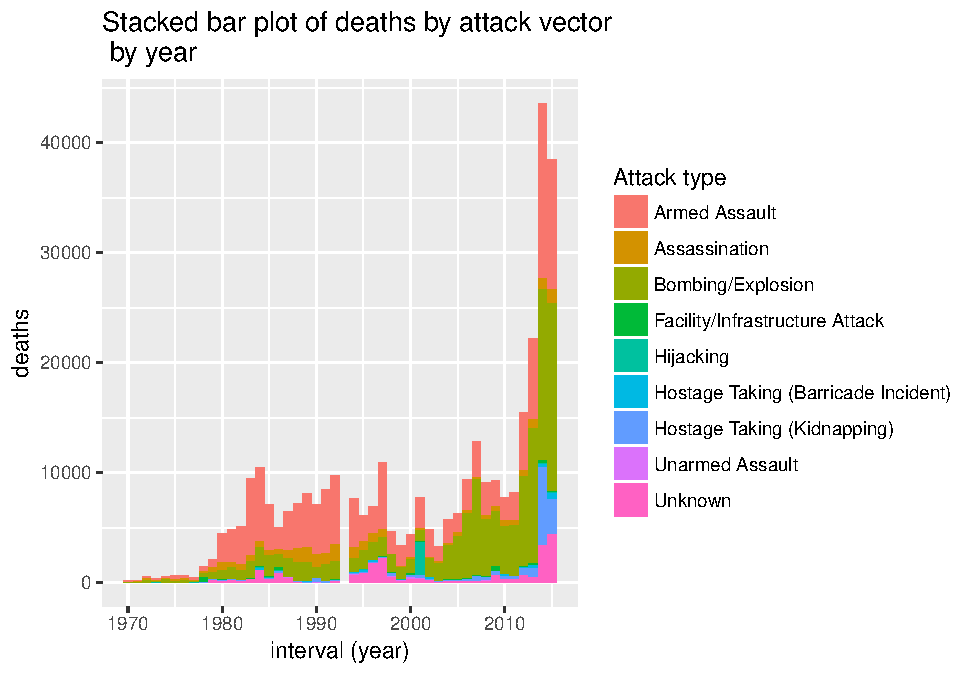
\includegraphics[width=10cm]{Peters_experiment_markdown_files/figure-latex/unnamed-chunk-7-1.pdf}
\caption{Stacked bar plot interval(year) of deaths by regions}
\label{fig:stackbaryearattackvector1}
\centering
\end{figure}

A similar trend is observed when we just look at the Middle east, with the dominating attack vector type being bombings and explosions figure~\ref{fig:stackbaryearattackvectormideast}.

\begin{figure}[t]
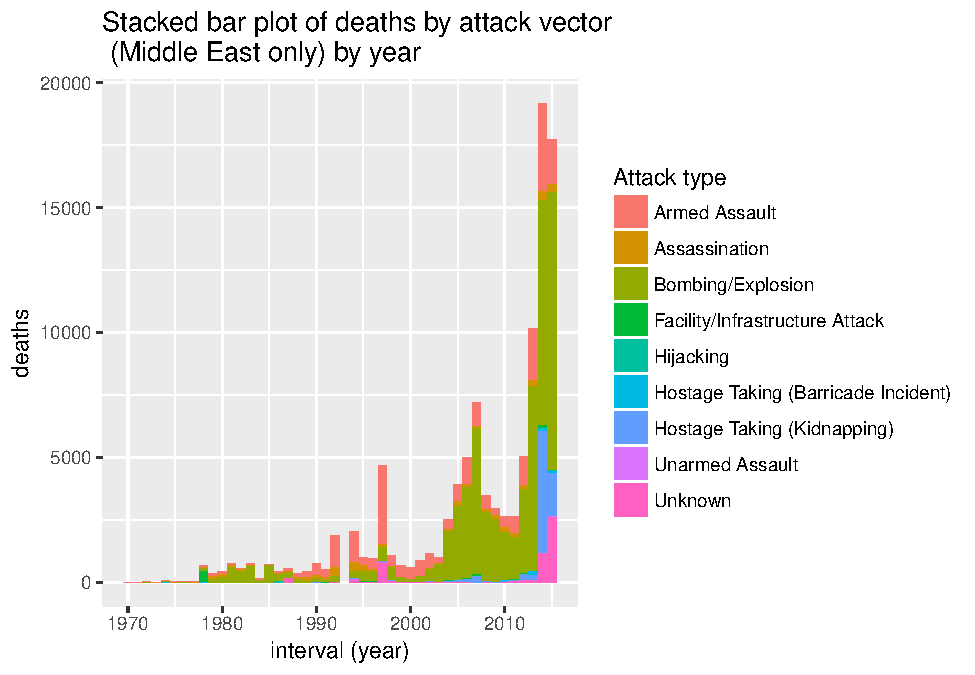
\includegraphics[width=10cm]{Peters_experiment_markdown_files/figure-latex/unnamed-chunk-8-1.pdf}
\caption{Stacked bar plot interval(year) of deaths by weapon type in the Middle East and North Africa}
\label{fig:stackbaryearattackvectormideast}
\centering
\end{figure}

When visualizing by attack type by interval year a clear pattern emerges. Up until the early 2000's the dominant weapon type used was firearms, however after this period explosives began to be the pre-eminent attack type (see figure~\ref{fig:stackbaryearweaptype}). 

\begin{figure}[t]
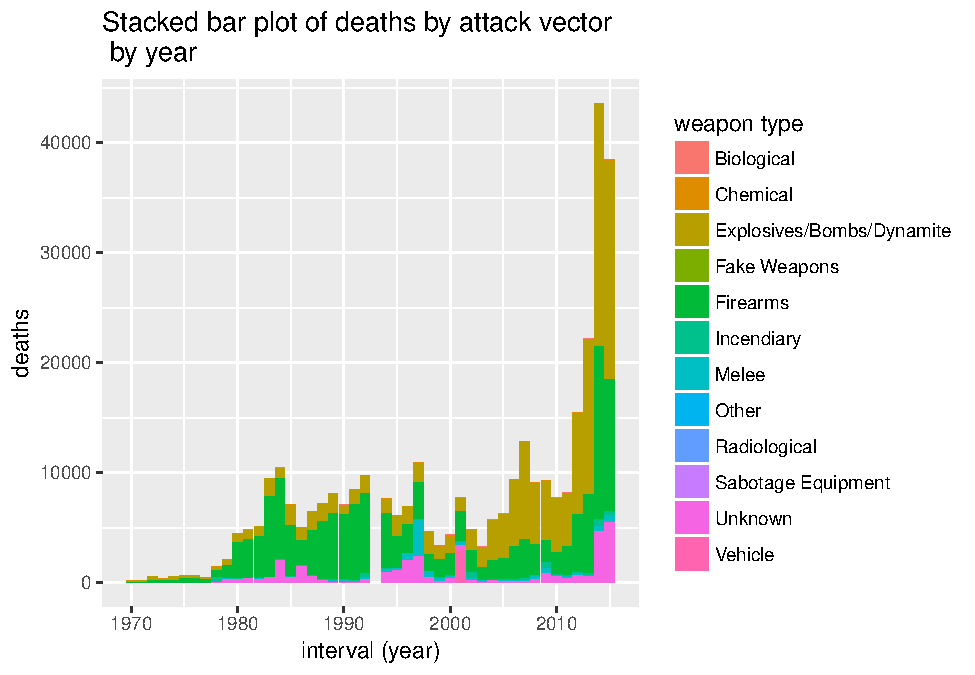
\includegraphics[width=10cm]{Peters_experiment_markdown_files/figure-latex/unnamed-chunk-9-1.pdf}
\caption{Stacked bar plot interval(year) of deaths by attack type}
\label{fig:stackbaryearweaptype}
\centering
\end{figure}

\subsection{Visualizing deaths by country and decade 
type}\label{viewing-deaths-by-attack-vector-type}

Previously the relationship by year and region had shown a regio-temporal shift in death due to terrorism (see section~\ref{sec:evteryearmonth}). By creating a stacked choropleth (figure~\ref{fig:choroplethdecade}), the number of deaths by decade (1970's, 1980's, 1990's, 2000's, 2010's) are visualized as a stacked choropleth, see figure~\ref{fig:choroplethdecade}. Again the regio-temporal shift in deaths can be seen. In the 1970's terrorism was not particularly associated with no one particular region. Britain, Spain, Italy, USA, Nicaragua, Colombia, Philippines and Argentina, show the largest number of deaths due to terrorism. In the 1980's a clear regio-specific pattern can be seem concentrated in Central and South America, particularly in Nicaragua, Guatemala and Colombia.

In the 1990's again no clear regio-specific pattern is seen with deaths due to terrorism being widely dispersed through out the World, though large scale deaths due to terrorism persisting in Colombia and Ecuador, Algeria emerging as a prominent country along with Southern Africa particularly (Angola, Mozambique and  South Africa) and Turkey and Russia. 

The 2000's sees a large increase in deaths in the US, Iraq, Russia, Afghanistan and Pakistan, but shows large decreases in India and Algeria. As well as a large decrease of terror from Southern Africa and Columbia and Ecuador.

\begin{figure}[t]
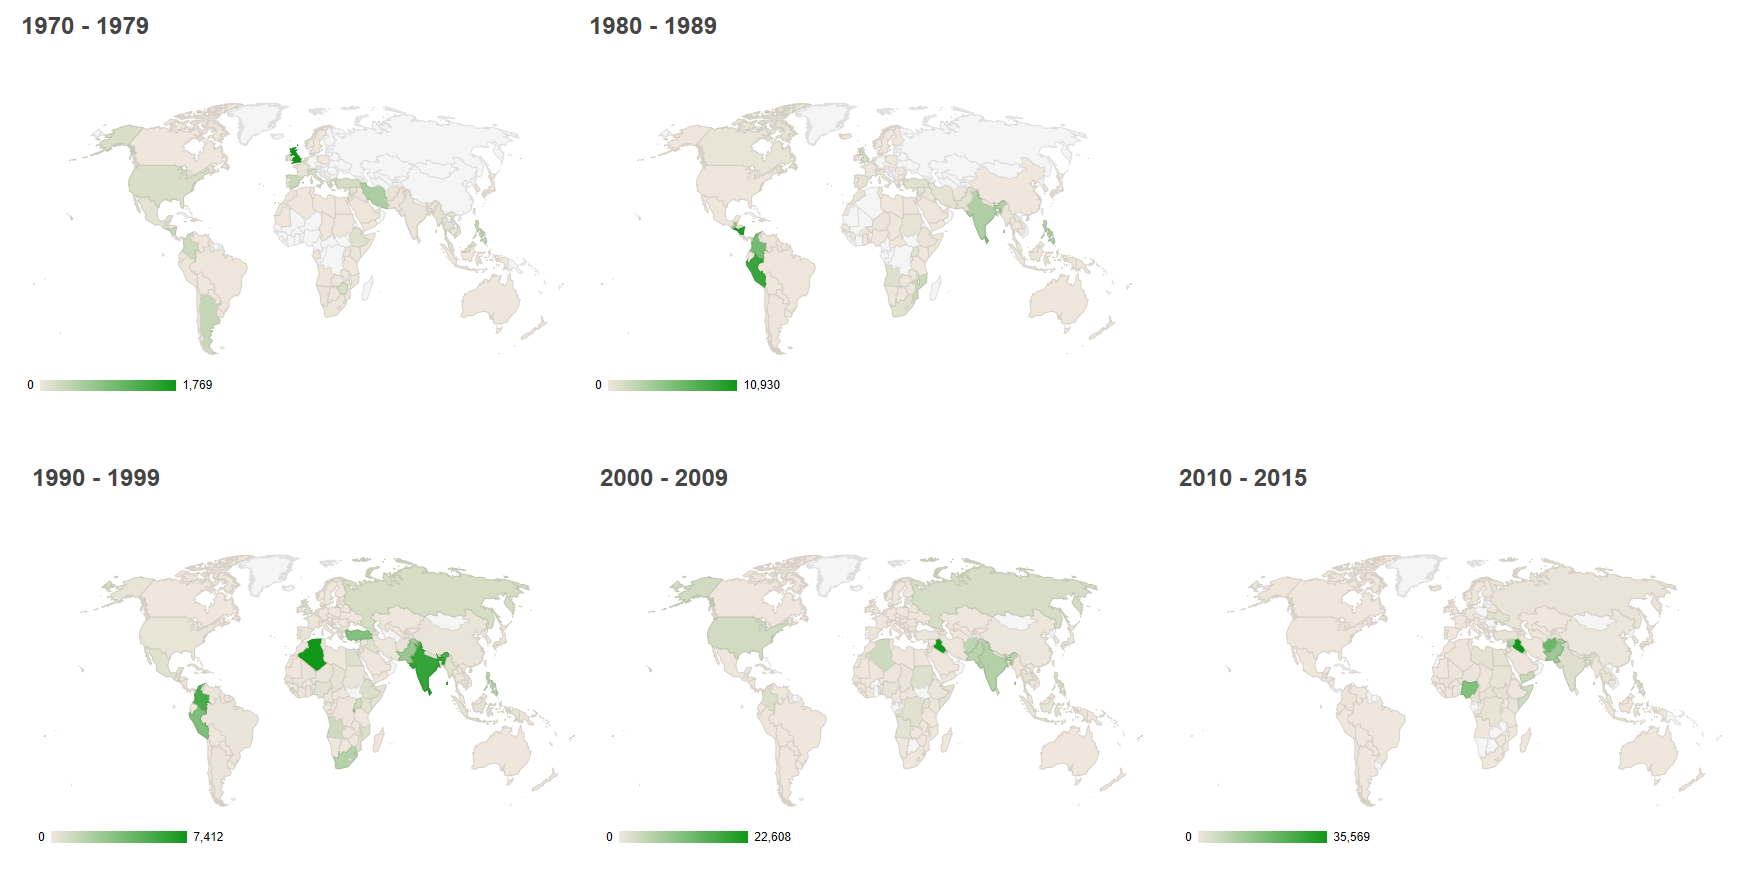
\includegraphics[width=15cm,height=15cm]{Peters_experiment_markdown_files/figure-latex/Capture_Choropleth_By_Decade_Deaths.png}
\caption{A stacked choropleth showing deaths by decade due to terrorism.}
\label{fig:choroplethdecade}
\centering
\end{figure}

\subsection{Visualizing deaths by rural urban 
categorization using K-means and Kernel Density estimation and interactive maps to create heatmaps} \label{viewing-deaths-by-K-means_Iraq_Syria}
In the previous sections(\ref:{section:viewing-deaths-by-attack-vector-type} and \ref{sec:evteryearmonth}) it could be quite clearly seen that South Asia (particularly Afghanistan) and the Middle East (particularly Iraq and Syria) were the predominant regions in terms of terrorist incidents and deaths. Iraq was chosen for further analysis as it has been (since the invasion of Iraq in 2003), the country which consistently ranks first in terms of deaths due to terrorism. Similarly, Syria since the Arab spring and the ensuing rebellion against the Assad regime of 2012 (\citep{dabashi2012arab}) which correlated with the rise of ISIS and the establishment of a caliphate across certain parts of Iraq and Syria, has also been a pre-eminent country in terms of deaths due to terrorism and incidents. 

These countries due to their predominance of terrorist activities, led to their selection for further analysis. Analysis at a finer grain (particularly spatial analysis) as opposed to the previous section which looked at quite broad trends can be carried out by using a combination of K-Means clustering, kernel density estimation and interactive visualization. Iraq and Syria were further examined  and one of the experiments undertaken was to see if a  rural urban divide (are attacks focussed in one specific area or/and are they associated with rural or urban areas) exists. To do this, only incidents from Iraq and Syria were chosen and the data was also limited to incidents that occurred in Syria and Iraq for 2015. 
Density estimation creates a fundamental estimate of the probability density function, kernel density estimation creates a smooth kernel function for all data points then aggregating these to get a density estimate. The fundamental kernel estimator is given by the equation \ref{eq:eq1kernelest}.

\begin{equation} \hat{f}_{kde} = 1/n \sum^n_{i=1} K((x-x_i)/h) \label{eq:eq1kernelest}  \end{equation}

\begin{equation} MISE(\hat{f})=E[\int(\hat{f}(x)-f(x))^2 \ dx]
\label{eq:eq1l2risk}  \end{equation}
Where:
\begin{itemize}
\item[]  Where $K$ is the kernel which is a symmetric, positive function which sums to one. Typical kernel function are uniform triangle, normal and cosine.
\item[]  Where $h$ is the bandwidth which is a smoothing parameter, large bandwidths create extremely smooth estimates while the  converse is true for small bandwidths which produce noisy estimates, as the smoothing tends to impact the estimates much more so than the choice of kernel, it is imperative to determine the optimum bandwidth. The bandwidth is usually chosen by reducing to a minimum the mean integrated square error, given by the equation \ref{eq:eq1l2risk}.
\end{itemize}

The bkde2d function of the Kernsmooth package is used to calculate the 2d kernel density estimate based upon the WGS84 coordinates of the terrorist incidents, linear binning is then used to create a series of bin counts and a 'Fast Fourier Transform (FFT)' is then utilized to carry out a series of discrete convolutions. A bivariate Gaussian kernel concentrated at the specific location and the heights of the kernel scaled by the bandwidths are then calculated and aggregated at every datapoint. This allows the creation of heatmaps by overlaying the density estimates on a map created using leaflet. The resulting map which overlays the points of the density estimates shows that in Iraq the incidents are largely concentrated around Baghdad while in Syria the incidents appear to be concentrated around the city of Allepo, figure~\ref{fig:iraqsyriakde}. To gain a greater understanding of the spatial distribution of incidents K-Means clustering was also used.

K-means clustering aims to divide a number of into k number of clusters and is one of the easiest to understand and popular implementations of clustering. The number of clusters is decided apriori, metrics can be used to guide the choice of K which minimize inter observation distance within clusters and maximize the distance between clusters. Such metrics include Davis Bouldin index \citep{davies1979cluster}. Alternately useful values for K can be chosen on whether the clusters make sense to the analyst based on expert knowledge. The algorithm can be summarized using the subsequent stages:
\begin{enumerate}
\item K points are arranged into the space characterized by the observations that are being clustered. These points are defined as the first cluster centroids.
\item For all observations they are assigned to the cluster with the nearest centroid.
\item Upon all observations being designated to a particular cluster, the location of the cluster centroids are determined.
\item Stages 2 and 3 are repeated until the centroids no longer change position. This produces a separation of the objects into groups from which the metric to be minimized can be calculated.
\end{enumerate}
Succinctly put, the K-Means algorithm goal is to minimize an objective function a squared error function given by the formula \ref{eq:eq1kmeans}, 

\begin{equation} J=\sum_{j=1}^{k}\sum_{i=1}^{n}\left \| x_{i}^{j} - c_{j} \right \|^{2} \label{eq:eq1kmeans}  \end{equation}

Where the formula \ref{eq:eq1kmeans} represents the distance metric between a specific observation and the cluster centre. 

\begin{equation} \| x_{i}^{j} - c_{j} \|^{2}  \label{eq:eq2kmeans}  \end{equation}

In the case of clustering  a set of longitude/latitude locations are utilized to calculate a distance matrix. This distance matrix is calculated by use of the great circle distance which is calculated for all couples or pairings of longitude/latitude (which locate a specific terrorist incident) using the haversine method (equation \ref{eq:haversine1}) where \textit{h} is haversine (equation \ref{eq:haversine2}). Solving equation \ref{eq:haversine1} is done by applying the inverse of the haversine equation and equation \ref{eq:haversine3}) is derived.  

\begin{equation} d = r hav^{-1}(h) - 2r\arcsin(\sqrt{h})  \label{eq:haversine1}  \end{equation}

\begin{equation} hav(\frac{d}{r}) =hav(\varphi_{2}-\varphi_{1})+cos(\varphi_{2})hav(\lambda_{2}-\lambda_{2})  \label{eq:haversine2}  \end{equation}

\begin{equation} d=2r \arcsin(\sqrt(sin^{2}(\frac{\varphi_2-\varphi_1}{2})+cos(\varphi_2)sin^{2}(\frac{\lambda_2-\lambda_1}{2}))  \label{eq:haversine3}  \end{equation}

Where:
\begin{itemize}
\item[]  $hav$ is the haversine function given by $hav(\theta)=sin^2(\frac{\theta}{2})=\frac{1-cos(\theta)}{2}$
\item[] r gives the radius of the sphere.
\item[] $\varphi_1, \varphi_2$: represent latitude of observation 1 and latitude of observation 2, in radians, note in fields the rdist.earth function used to calculate the distance matrix in the fields package \ref{fields2015Nychka}, carries out a conversion from WGS84 \citep{misra1996integrated} to radians.
\item[]  $\lambda_1,\lambda_2$: represent the longitude of observation 1 and observation of point 2, in radians, note again in fields the rdist.earth function carries out a conversion from WGS84 \citep{misra1996integrated} to radians.
\end{itemize}

Contrasting the analysis from the kernel density estimate based visualization and the clustering exercise provides some interesting insights.
   
From figure~\ref{fig:iraqsyriakde}, it can be seen from the overlaying of the binned kernel density of the probability of incidents (estimated from latitude and longitude of the incidents) that the incidents in Iraq are concentrated in Western Iraq specifically around Baghdad and the Sunni triangle \citep{rand2015iraq} of Tikrit, Ramadi and Baghdad which are the most densely populated areas of Iraq and inhabited mostly by Sunni Muslims, which became the centre for armed resistance and Sunni opposition to the 2003 of Iraq \citep{hashim2005insurgency}, figure~\ref{fig:kmeansSyriaIraqSunniTriangle}. In Syria the incidents are concentrated around Aleppo, Homs, Latakia and Damascus. The clusters relating to these highly urbanized areas are categorized as being tightly grouped together as opposed to the clusters covering the Iraqi Western Desert and the Syrian Eastern Desert which are sparsely populated, figure~\ref{fig:kmeansSyriaIraq}.

\begin{figure}[t]
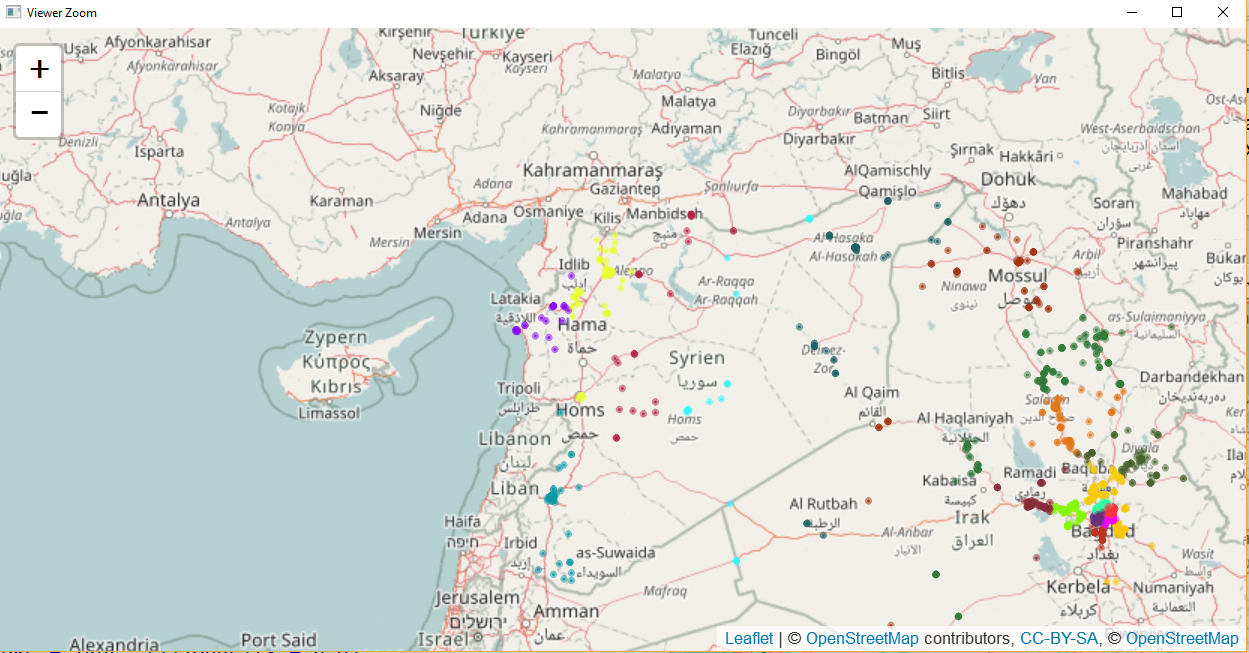
\includegraphics[width=15cm,height=15cm]{Peters_experiment_markdown_files/figure-latex/Capture_Kmeans_Leaflet_2015_Deaths_Iraq_Syria_K20.png}
\caption{Clustering of Terrorist incidents in Syria and Iraq}
\label{fig:kmeansSyriaIraq}
\centering
\end{figure} 

\begin{figure}[t]
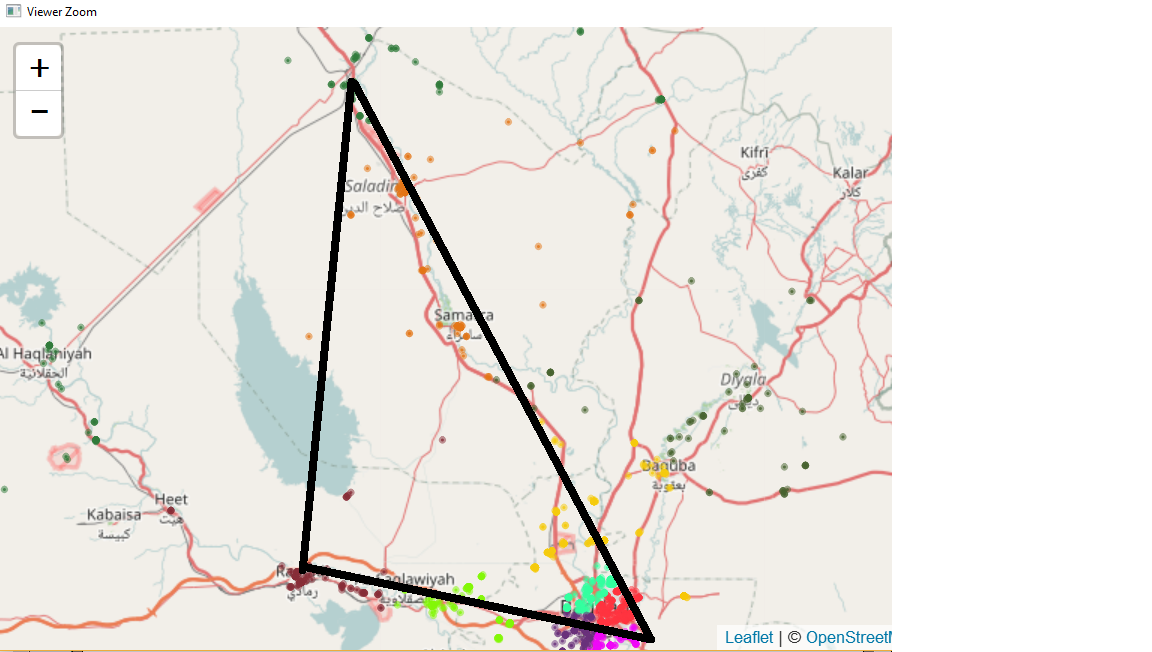
\includegraphics[width=15cm]{Peters_experiment_markdown_files/figure-latex/Capture_Kmeans_Leaflet_2015_Deaths_Iraq_Syria_K20_Sunni_Triangle_2.png}
\caption{Clustering of Terrorist incidents in Syria and Iraq, centred on the Sunni triangle}
\label{fig:kmeansSyriaIraqSunniTriangle}
\centering
\end{figure}

\begin{figure}[t]
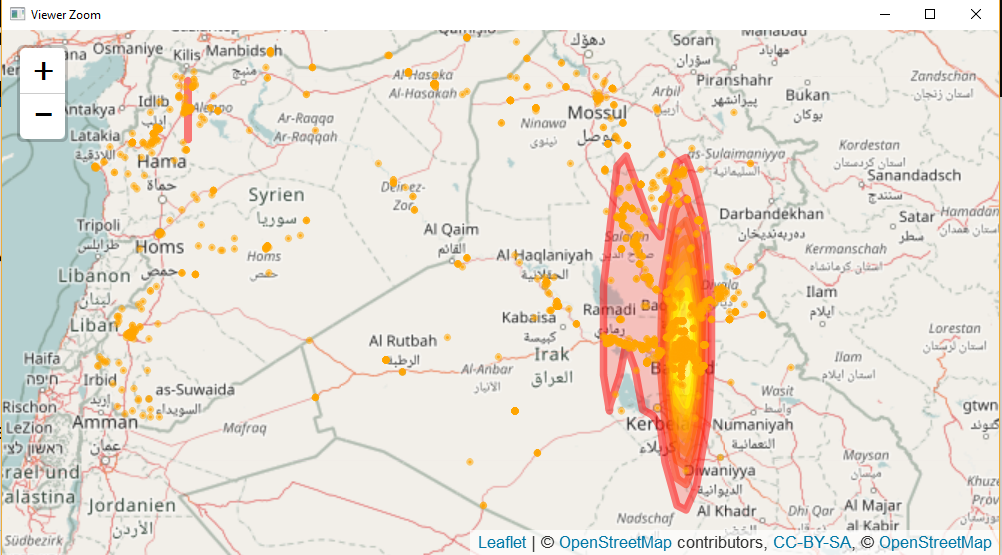
\includegraphics[width=15cm]{Peters_experiment_markdown_files/figure-latex/Capture_KDE_Leaflet_2015_Deaths_Iraq_Syria.png}
\caption{Heatmap of terrorist incidents in Syria and Iraq}
\label{fig:iraqsyriakde}
\centering
\end{figure}
 
\section{The use of dimension reduction techniques and clustering in understanding the GTD}\label{viewing-deaths-by-attack-vector-type} 

While the previous section largely utilised simple descriptive data visualizations or kernel density estimation and cluster analysis to uncover underlying patterns in the data, these visualizations are limited in the number of data dimensions they can encode. To overcome this dimension reduction techniques (particularly Correspondence Analysis (CA) and Multiple Correspondence Analysis (MCA)) are used to reduce the data down from n dimensions to a more lower level while still maintaining the underlying structure in the data. These techniques can also be considered descriptive analytical techniques but are not limited to a low number of dimensions. CA (and MCA) is used in conjunction with D3 \citep{bostock2012d3} based interactive visualizations, using plotly \citep{plotlymanual2016} accessed through the R plotly package to create the bi-plots of the output of the analysis. This is done to aid navigation of the data and to ease understanding of many level categorical variables, which may appear crowded otherwise and difficult to understand. The reason correspondence  analysis is so appropriate to the study is the type of  data, which is largely categorical in nature. 

CA is a multivariate statistical technique which is notionally similar to the more well known dimension reduction technique, principal component analysis (PCA). It is used as a statistical visualization technique for envisaging the associations (note the phrase correspondence comes from the french 'Analyses des Correspondances' where correspondence signifies a "system of associations" which exist between the different items which make up the two sets of data) or relationships between the different levels of a two way cross-tab table \citep{husson2010exploratory}. Two-way contingency tables are utilized in statistics to show how the perceived associations of two attributes (represented as rows and columns) and displayed as cell frequencies of a matrix. An archetypical task within inferential statistics is to ascertain the level of association between levels of one variable and levels of the other variable. CA transforms the data held within rows and columns of a two way contingency table into a lower dimensional space so that the points of the rows and columns in the lower dimensional space are representative of their associations in the table. The mathematics of CA is briefly explained previously in section \ref{sec:synglobalter}.  

\subsection{Correspondence analysis of weapon type by year}\label{viewing-deaths-by-weapon-vector-type-CA}

CA was used understand better both the relationship year and weapon type. The contingency table of number of deaths by years and weapon type is shown in table \ref{tab:weaponsyear}.

Correspondence analysis is carried out and visualized in the form of a biplot using a standard static plot created using using ggplot, however the static nature of the plot does not aid in their interpretation due to over-crowded nature of visualization, this is illustrated in figure \ref{fig:biplotweaponsyears}. When Plotly (D3 based interactive visualization tool) is used to create the visualizations, the resulting visualizations can be configured to zoom in and out (the zoomed out visualization is shown in figure~\ref{fig:biplotweaponsyearsplotlyzoomout}) and particular regions (of the visualization) can be highlighted and it is possible to clearly ascertain what associations if any exist (see figure~\ref{fig:biplotweaponsyearsplotlyzoomin}). From the 2000's on explosives bombs and dynamite have been the dominant, while vehicular attacks do not appear to be strongly associated with any particular year or epoch. While the use of Firearms seem to be particularly popular in the 1980's and very strongly associated with 1996.
 
\begin{figure}[t]
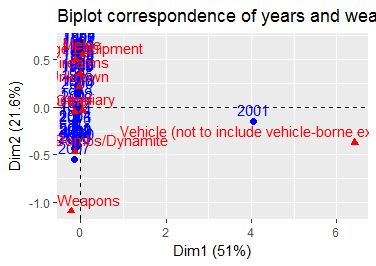
\includegraphics[width=15cm]{Peters_experiment_markdown_files/figure-latex/Rplot_CABIPLOT.png}
\caption{Biplot CA of contingency table of deaths by weapons and year.}
\label{fig:biplotweaponsyears}
\centering
\end{figure}

\begin{figure}[t]
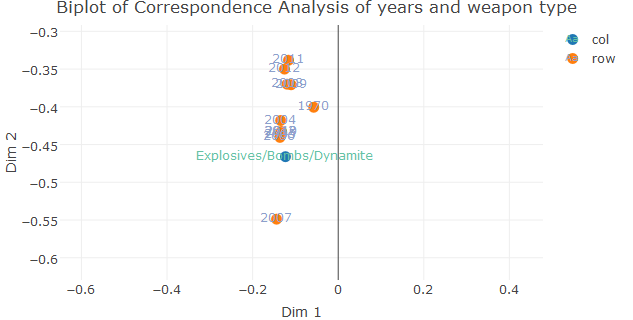
\includegraphics[width=15cm]{Peters_experiment_markdown_files/figure-latex/biplot_zoomin.png}
\caption{Biplot CA of contingency table of deaths by weapons and year, created using Plotly, zoomed in.}
\label{fig:biplotweaponsyearsplotlyzoomin}
\centering
\end{figure}

\begin{figure}[t]
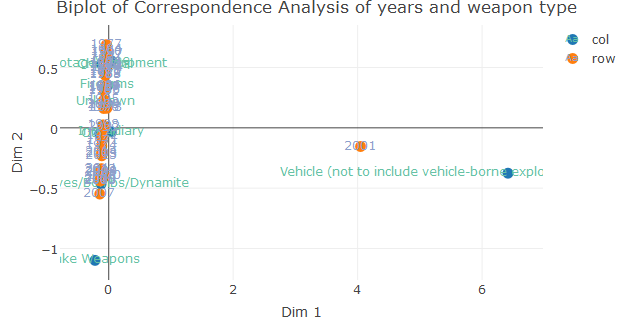
\includegraphics[width=15cm]{Peters_experiment_markdown_files/figure-latex/biplot_zoomout.png}
\caption{Biplot CA of contingency table of deaths by weapons and year, created using Plotly, zoomed in.}
\label{fig:biplotweaponsyearsplotlyzoomout}
\centering
\end{figure}

\subsection{Correspondence analysis of attack type by year}\label{viewing-deaths-by-attack-vector-type-CA}

CA was used to understand better both the temporal relationship between year and attack type. The contingency table of number of deaths by years and weapon type is shown in table \ref{tab:attacksyear}. From the Biplot , it can be seen that bombings and explosions are strongly associated with 2005 and 2006. Hostage taking or barricade incidents are strongly associated with 1974 and 1998 infrastructure attacks are strongly associated with 2002 and assassinations.

\begin{figure}[t]
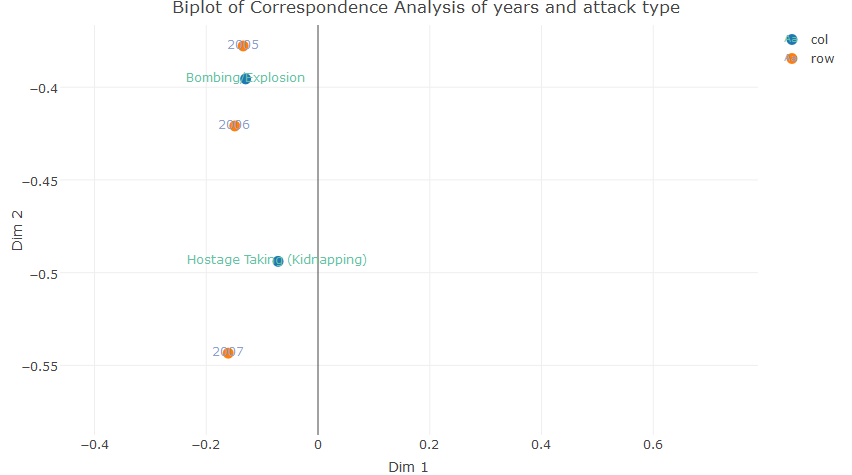
\includegraphics[width=15cm]{Peters_experiment_markdown_files/figure-latex/biplotexlosions.png}
\caption{Biplot CA of contingency table of deaths by attack type and year, created using Plotly, zoomed in to show associations between explosions  and years they occurred.}
\label{fig:biplotattacktypeca1}
\centering
\end{figure}
\begin{figure}[t]
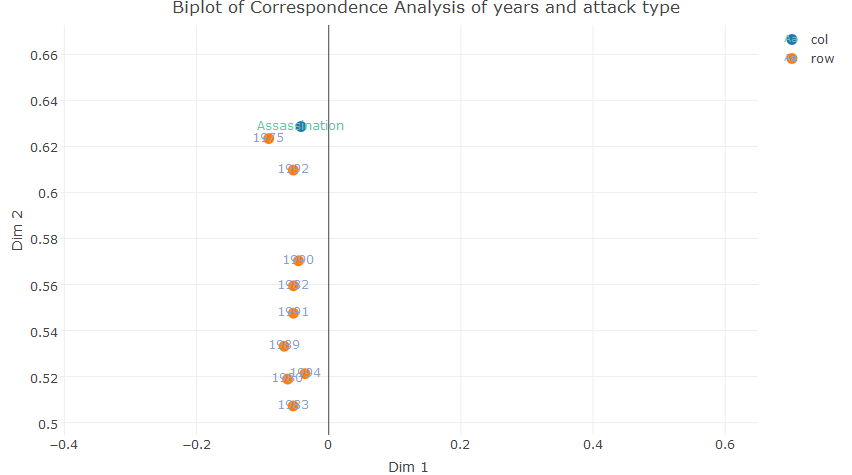
\includegraphics[width=15cm]{Peters_experiment_markdown_files/figure-latex/assassinationbiplot.png}
\caption{Biplot CA of contingency table of deaths by attack type and year, created using Plotly, zoomed in to show associations between assassinations and years they occurred.}
\label{fig:biplotattacktypeca2}
\centering
\end{figure}
\begin{figure}[t]
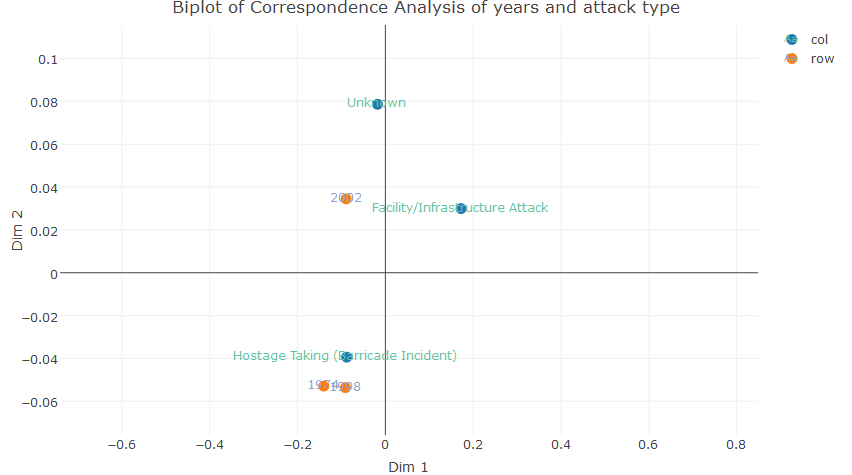
\includegraphics[width=15cm]{Peters_experiment_markdown_files/figure-latex/hostagetakingbiplot.png}
\caption{Biplot CA of contingency table of deaths by attack type and year, created using Plotly, zoomed in to show associations between hostage taking and years they occurred.}
\label{fig:biplotattacktypeca3}
\centering
\end{figure}

\subsection{Multiple Correspondence analysis of terrorist incidents the GTD by year}\label{viewing-deaths-by-attack-vector-type-MCA}

Multiple correspondence analysis (MCA) is an expanded form of correspondence analysis which accommodates the analysis of the relationships between a number of categorical variables. MCA is also known by a number of synonyms including  optimal scaling or appropriate scoring. Methodologically MCA is carried out by carrying out a atypical CA of an indicator matrix (this is a matrix were the values of individual cells take on values or either 0 or 1). Upon carrying out the CA, the percentages of the explained variance are revised and the inter-point distances which result from the CA are adapted to account for this. Multiple correspondence is an extension of correspondence analysis that allows analysis of multiple variables. Instead of analysis counts of deaths, analysis of terrorist incidents is carried out, the data is also filtered to include only incidents from 'North Africa and the Middle East'. The benefit of using MCA is that the relationship between multiple levels of multiple categorical variables can be examined. A number of incites can be gained from examining the bi-plot (see figure~\ref{fig:biplotmca}), examining the bi-plot it can be seen that:
\begin{itemize}
\item  There is strong association between 1974 and terrorist attacks on non state militia or terrorists.
\item Unarmed assaults are strongly associated with chemical weapons use.
\item 2003 are strongly associated with attacks against government, while 2009 shows a strong association with attacks targeting police.  
\item 1994 is strongly associated with attacks using weapon types sabotage equipment and mellee weapons against facilities and infrastructure.
\end{itemize}

\begin{figure}[t]
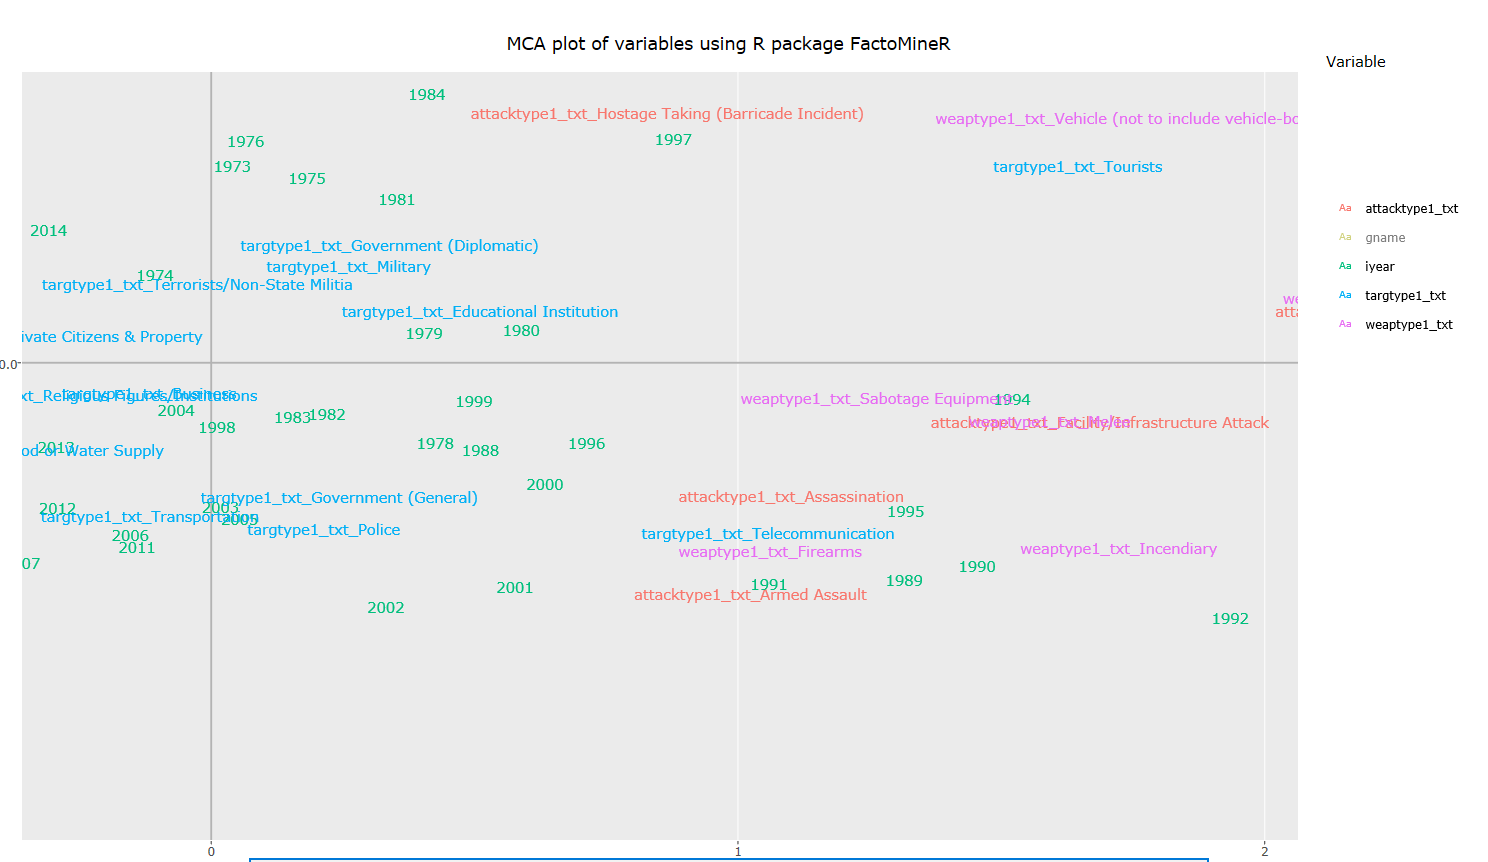
\includegraphics[width=15cm]{Peters_experiment_markdown_files/figure-latex/newplot3.png}
\caption{Biplot of MCA of incidents by attack type, weapon type, target type, group name and year, created using Plotly, zoomed in to show associations between hostage taking and years they occurred.}
\label{fig:biplotmca}
\centering
\end{figure}

\section{Preliminary modelling techniques to gain a temporal understanding of terrorism}
Both Poisson regression and HMM's (Hidden Markov Models) were employed to gain a better understanding of temporal nature of terrorism. While the models utilized are relatively simple they are to used aid in the understanding of the temporal nature of terrorism and also to ascertain how events not held in the GTD database can be used to explain the events held within. To do this two separate preliminary studies are carried out, these are:
\begin{itemize}
\item Poisson regression is used to model the count of deaths due to terrorism in Iraq in terms of months and major events over the period 1970 to 2015. These events are  represented in the time-line chart shown in figure~\ref{fig:timelineiraq}. The aim of carrying out the Poisson regression analysis is to identify what events are affecting the count of deaths due to terrorism. 
\item HMM's are used to model the number of deaths as a time series and the resulting transition state probabilities delivered by the model are used to determine whether the country is in a state of insurgency (transition probability of being in a period of large numbers of daily deaths is high) or in a state of 'relative calm'  (transition probability of being in a period of low numbers of daily deaths is high).
\end{itemize}

\section{Poisson, Quasi Poisson, Negative Binomial, Linear  and Robust (of log transformed)  regression of deaths due to terrorism in Iraq by month}

Iraq has had a Tumultuous history and in recent years has seen a massive increase in terrorism since the US invasion to overthrow Saddam Hussein's Ba'athist regime, this is visualized in figure~\ref{fig:timelineiraq}. From the time-line plot, one can see a number of key events in Iraq and when the event, both on the time-line but also in terms of the reign of the different governing bodies in Iraq, US and Great Britain occurred. From the time line one can see the following:
\begin{enumerate}
\item The invasion and the US Troop surge took place under Bush regime. The Post surge period and initiation of the draw down of US and NATO troops from Iraq took place.  
\item  Under the Obama administration, the Post surge period continuing into the drawdown of US troops to the eventual pullout of US and NATO troops took place. The Obama administration was also in place during the rise of ISIS and also the replacement of the Nouri Al Maliki government, which was largely viewed as ineffective (both in terms of effectively managing the country and also the fight against Al Qa'ida), \citep{simon2008price} and \citep{kuoti2016exclusion}.
\end{enumerate}

\begin{figure}[t]
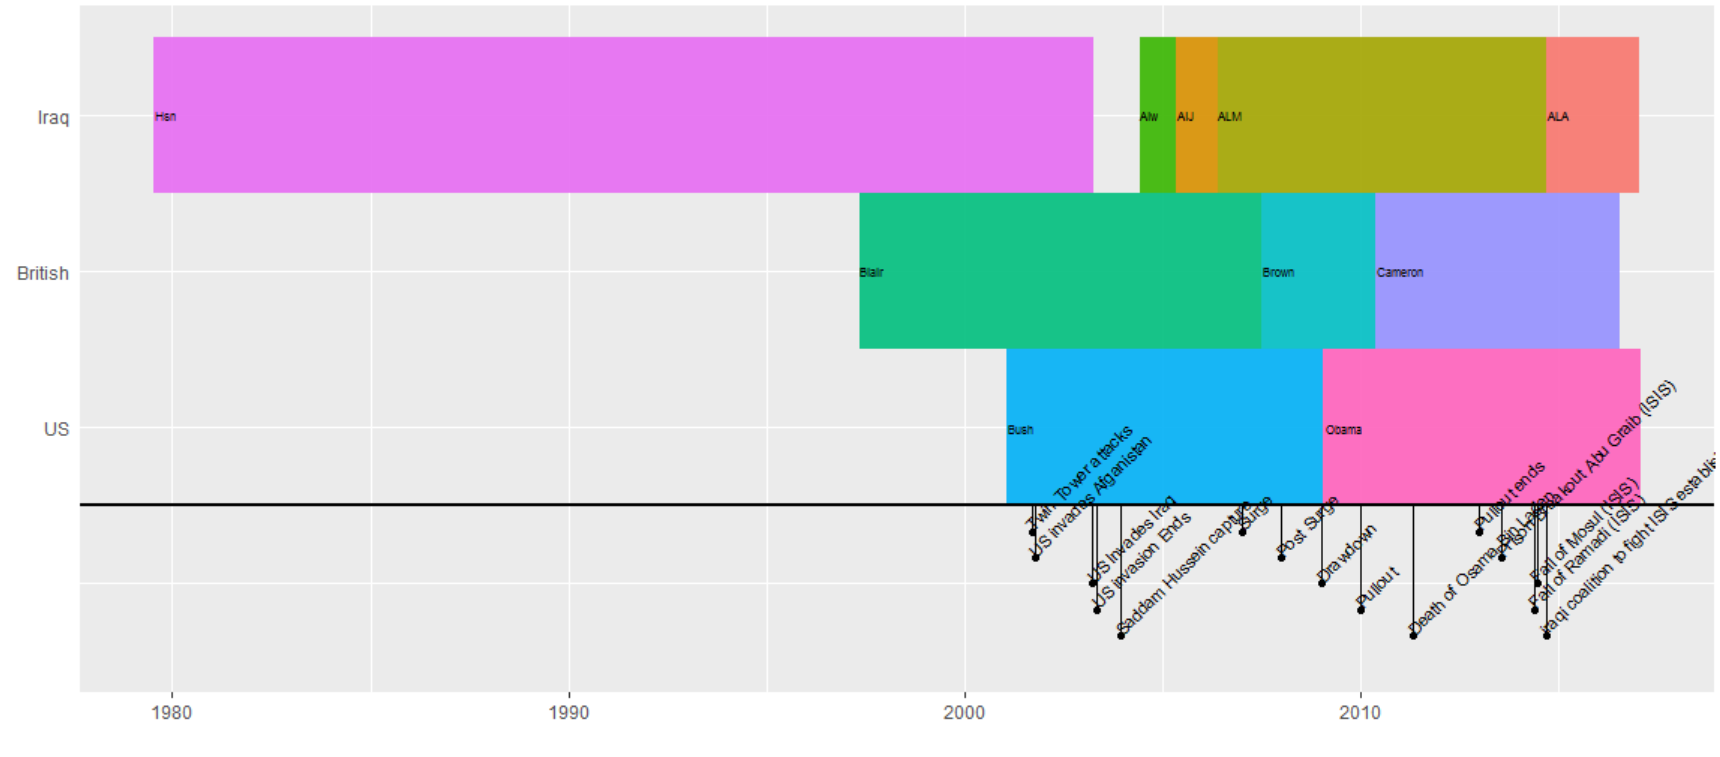
\includegraphics[width=15cm]{Peters_experiment_markdown_files/figure-latex/CaptureTimelineIraq.png}
\caption{Timeline of Iraq post and pre invasion (2003}.
\label{fig:timelineiraq}
\centering
\end{figure}

Over the same period the deaths due to terrorism is shown in figure~ \ref{fig:deathsiniraq}. From the plot of deaths by years for Iraq not only it is clear that only after the invasion of Iraq, did the number of deaths due to terrorism rise. It's also clear from the bar chart that the outbreak of deaths that occurred increased sharply from 2003 to 2007, peaking during the year of the US troop surge.  

The preceding years upto 2012 sees a fall off in the number of deaths over this period followed by rise of ISIS \citep{sekulow2015rise} and the resulting civil war in neighbouring Syria, which sees a large increase. 

\begin{figure}[t]
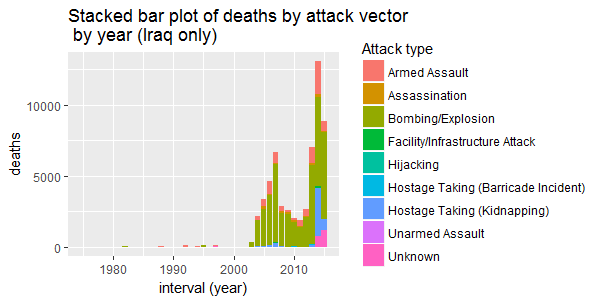
\includegraphics[width=15cm]{Peters_experiment_markdown_files/figure-latex/Rplot01IraqDeaths.png}
\caption{Timeline of Iraq  and US and British presidents and major events since the Iraq invasion.}
\label{fig:deathsiniraq}
\centering
\end{figure}

Poisson regression was first used to model the monthly death totals due to terrorism in Iraq. Poisson regression is used to model count data, counts are positive integers which represent the number of events which have occurred (in this case it represents the number of deaths due to terrorism). The density distribution for a Poisson distribution is given by the following equation (equation~\ref{eq:poisseqdens}).

\begin{equation} f(y:\mu)= \frac{exp(-\mu)\cdot \mu^y}{y!}  \label{eq:poisseqdens}  \end{equation}

In modelling such events, a Poisson distribution is appropriate as the mean is always greater than 0. Both the mean and variance of the distribution can be shown to be equal. As the variance and the mean are equal anything that affects the mean will also affect the variance. In Poisson regression the logarithm of the dependent variable is linked or connected to a linear function of the explanatory variables in such way that it is given by (equation~\ref{eq:poisseq}).

\begin{equation} log(y)=Intercept+b_1x_1+b_2x_2...b_nx_n   \label{eq:poisseq}  \end{equation}

Specifically a Poisson regression model, estimates the response variable, the log outcome rate as a linear function of a group of independent variables. Poisson regression makes a number of assumptions about the data. These are:

\begin{itemize}
\item The variable you are trying to predict, the response variable is count data and must be positive.
\item There are one or more predictor variables that are continuous, ordinal or categorical.
\item Independence of observations should be observed in the data, in other words, i.e one observation cannot inform another observation.
\item The distribution of counts being modelled should follow a Poisson distribution. This can be observed by checking the dispersion (for over and under dispersion) of the model. Over dispersion is  were a larger amount of variability is observed in the response variable than is seen in the predicted response using the statistical model. Under dispersion is where there is less variability in the response variable than in the predicted response.
\end{itemize}

The data was modelled using US and Iraqi president term data, US interventions, terrorist interventions and month since 1970 (when the precursor to the GTD, the PGIS began). 
The dataset was created from the GTD by joining it to the CRS (Congressional Research Service) reports for congress on us troop levels (which were used to assign the Surge, Post surge, Pullout and Post pull-out time periods) along with CRS reports \citep{peters2016department}, \citep{belasco2009troop} and \citep{o2007us}, and information regarding inherent resolve (US led coalition against ISIS), \citep{fischer2015guide}. US and Iraqi presidential terms were scraped from Wikipedia. The dataset is created by aggregating the monthly death count due to terrorism in Iraq aggregated by Month, Iraqi President, US President, US troop levels or intervention and major insurgent/terrorist interventions.

The summary table (see table~\ref{tab:poiss})  shows that the model may suffer from a number of a problems. The first parameter of note is the residual deviance of the model. This can be used to calculate a goodness of fit test by carrying out a goodness-of-fit chi-squared test. The null hypothesis of the test is that the model has been specified in a correct manner, however when the test is run,  a low probability is obtained  approximately 0, therefore rejecting the null hypothesis that the model is correctly specified. On discovering the Poisson model (and the related Quasi-Poisson and Negative binomial to less an extent) were incorrectly specified, a linear model (as well as a robust linear regression model) on log transformed count data was trialled instead (these suffered from their own problems due to the transformation on the data required to meet the specifications of the model). Also a dispersion test is ran and the test clearly shows that the model is strongly over-dispersed.

As stated in the assumptions of Poisson GLMS, for a Poisson GLM the variance and mean are equal, the disperion test \citep{AerRPack} examines whether this assumption (the data is equidispersed) is true or not against the alternative hypothesis  that the variance is equal to the mean \ref{eq:disptest1}.

\begin{equation} VAR[y] = \mu + \alpha * trafo(\mu)   \label{eq:disptest1}  \end{equation}

Where alpha is greater than 0 the model is said to be over-dispersed. This test confirmed that the  model suffered from over dispersion.  Quasi-Poisson regression was used, this methodology does not restrict the dispersion parameter $phi$ to be 1, but is instead  calculated from the data. This has the effect that the coefficient estimates that are calculated from the Poisson model being the same  but the inference from the model is  changed to take account for over dispersion. Examining the summary of the Quasi-Poisson, we can see that the residual deviance has not changed. The dispersion parameter which was forced to be 1 when fitting a Poisson regression model is now estimated to be 77.30, indicating over-dispersion. The summary information for both models (Poisson and Quasi Poisson) are shown in tables~\ref{tab:poiss} and \ref{tab:quassipoiss}. 

Another alternative tried was the negative binomial model which is another methodology for modelling count data \citep{ver2007quasi}. This methodology presumes a negative binomial distribution which comes about as a gamma mixture of different Poisson distributions. Its probability density can be estimated using the function~\ref{eq:negbin}:

\begin{equation}  f(y:\mu,\theta)=  (\frac{\Gamma(y+\theta)}{\Gamma(\theta)\cdot y!})\cdot \frac{\mu^y\cdot \theta^\theta}{(\mu+\theta)^{y+\theta}}  \label{eq:negbin}  \end{equation}
where:
\begin{itemize}
\item[] $\mu$ =  mean
\item[] $\theta$ = shape parameter
\item[] $\Gamma\cdot$ = is the gamma function
\end{itemize}

The negative binomial model is available in the MASS package \citep{venables2002random}. The negative binomial models makes the assumption that the conditional means and the conditional variances are the same. This inequality is accounted for by evaluating a dispersion parameter which is held constant when using Poisson regression. In the case of the negative binomial model the theta value is estimated to be 1.035329979.

From the data (table \ref{tab:negbin} and \ref{tab:poiss}) it can be seen that, twice the difference between log likelihoods of the Poisson model and the negative binomial model is observed of 14643 with a difference in degrees of freedom of 22, df=22-21=1. The large chi-squared value estimated from the difference in log likelihood would tend to suggests the negative binomial model, which estimates the dispersion parameter, is a more appropriate choice than the Poisson model. Also from examining the summary model of the Poisson (table~\ref{tab:poiss}), quasi-Poisson (table~\ref{tab:quassipoiss}) and negative binomial model (table~\ref{tab:negbin}) shows that the model with the lowest AIC is the negative binomial model (3011.1). However a goodness of fit test for the negative binomial model performed by comparing the residual deviance compared to the maximum deviance of a perfect model where the predicted values match exactly the observed values, gives a statistically significant result, due to the large residual difference. This would indicate that the model does not fit the data perfectly well (though it would appear to be a better fit than either the Poisson or quasi-Poisson model), so while the model may be wrong it may still be useful. Examining the table of regression coefficients for the negative binomial model (table~\ref{tab:negbin}), allows us to see which events were correlated (and having a statistically significant effect on the independent variable) with positive or negative effects on the numbers killed per month in Iraq. The post invasion the surge and the ISIS campaign 'soldiers Harvest' have positive regression coefficients which are statistically significant, indicating that these events are correlated with increases in deaths due to terrorism.  

Finally a linear model (and a robust linear model) was fitted using log transformed count outcomes and analysed using OLS regression \citep{UCLAPoiss}. Before carrying out the linear regression model the response variable is log transformed. The model is then created and the specification is checked by examining the fit output. The general linear f-test applied to our model tests the assumption that the fit of the intercept only model is decidedly less than that of the fit of the model trained. From the summary table the calculated F-statistic is 72.3 (on 20 and 255 degrees of freedom) and the resulting p value is $< 2.2e-6$, suggesting we reject the null hypothesis and accept the alternative hypothesis that the model fit is significantly better than that of the intercept only model. The $R^2$ value obtained from the model is  0.8501 and the residual standard error which is the positive square root of the mean square error, this is calculated to be 0.9778 on 255 degrees of freedom. The model output is shown in table~\ref{tab:linearreg}.To check if our model is specified correctly, a series of diagnostic plots are created to check for the following criteria :
\begin{itemize}
\item Linearity. The relationship between the predictor variables and the response is linear.
\item Homoescadicity. There should be no relationship between the variation in the predictor variables and the error.
\item Independence. The error values are not a caused by any neighbouring values.
\item The error term is normally distributed.
\end{itemize}

To check if the assumptions made by the linear model are met a number of diagnostic plots were used to judge if the assumption of the linear model were met. First a plot of the residuals versus the fitted values was plotted to check the linearity assumption, figure~\ref{fig:residualsdiag}. While no clear patterns are visible from the residuals versus fitted plot, the residuals are not evenly spread around the line but instead they are clustered together around the midpoint and either extremes of the horizontal line. However a u-shape indicative of a non linear relationship is not observed. 

Secondly a Q-Q plot is plotted to see if the residuals are normally distributed. A Q-Q plot is a plot used to check for normality, (see figure~\ref{fig:qqplotdiag}). By plotting the theoretical quantiles (for a normal distribution) against the actual one can see how well the residuals approximate the normal distribution. While very few points deviate from the line very much at either end of the line there is some deviation. Thirdly a scale location plot (figure~\ref{fig:scalelocationdiag}) is created to check for homoescadicity, i.e. that the residuals are spread out evenly across the different values of the predictors \citep{neter1996applied}. While the spread of residuals do not  spread out as much along the x-axis the horizontal red line is fairly straight and the residuals do appear to be randomly deposited. No Clear pattern is observed in the data and a sloped line either up or down indicating heteroescadicity is not observed. However at lower observed values there appears to be greater variation in the residuals, which may indicate heteroescadicity. Finally a residual versus leverage plot is run to check if any influential cases which may be present in the data are affecting the fit of our model and as such are extremely influential \citep{sall1990leverage}. If these points exist they are located in the upper and lower right hand corners. Cooks distance \citep{chatterjee2009sensitivity} which is used to check for the presence of outliers is denoted in Figure~\ref{fig:cookdistdiag}. From the leverage plot it would appear that some of the observations did posses a high amount of leverage which could effect our regression estimates. Instead of removing the points, a regression method was used which could cope better with any violations of the assumptions of the linear model, robust regression \ref{tab:robustreg}.

A robust regression analysis \citep{rousseeuw2005robust} was then run as a final step in case the linear model was correctly specified, (which from the diagnostic plots there did appear to be some concerns particularly regarding the presence of outliers). The model coefficients are shown in table~\ref{tab:robustreg}. 

Robust regression methods are created to be not overly sensitive by violations of assumptions by the underlying data-generating process (i,e outliers). The residual standard error (0.4984) on 255 degrees of freedom and the weighted $R^2$ value of 0.9590327. A robust F-test is computed for each predictor (to show the significance of each predictor) in the robust regression model and the output is shown in table~\ref{tab:robustreg}.

\begin{figure}[t]
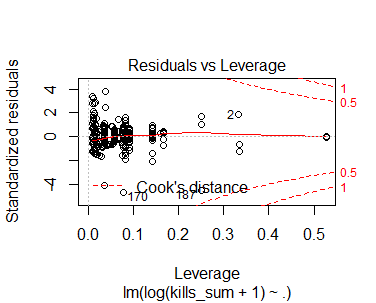
\includegraphics[width=15cm]{Peters_experiment_markdown_files/figure-latex/Rplot02_cooksdistance.png}
\caption{Cook distance diagnostic plot}.
\label{fig:cookdistdiag}
\centering
\end{figure}

\begin{figure}[t]
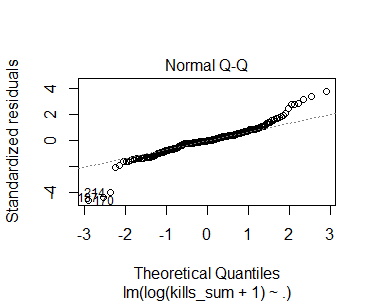
\includegraphics[width=15cm]{Peters_experiment_markdown_files/figure-latex/Rplot02_qqplot.png}
\caption{QQ plot diagnostic plot}.
\label{fig:qqplotdiag}
\centering
\end{figure}

\begin{figure}[t]
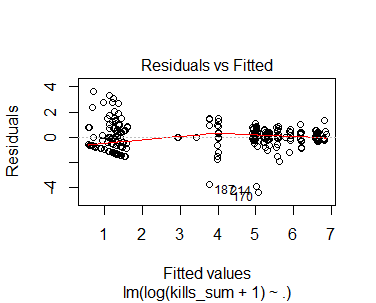
\includegraphics[width=15cm]{Peters_experiment_markdown_files/figure-latex/Rplot03_residuals_fitted.png}
\caption{Fitted residuals diagnostic plot}.
\label{fig:residualsdiag}
\centering
\end{figure}

\begin{figure}[t]
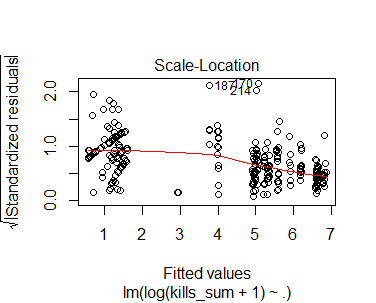
\includegraphics[width=15cm]{Peters_experiment_markdown_files/figure-latex/Rplot02_scale_location.png}
\caption{Scale location diagnostic plot}.
\label{fig:scalelocationdiag}
\centering
\end{figure}

A robust F-Test is then performed on each of the coefficients of the model to test the importance of the predictor variables. The values are listed in table~\ref{tab:robustregFtest}. From the table we can see that the variables that are significant level (at p $0.05$) are from Period 1 (which refers to periods of major US activity in Iraq) the surge and the post invasion period.  Period 2 (which relates  to periods of major activity by Insurgent groups) shows the ISIS soldiers harvest  campaign which was launched in August 2013 by ISIS to be significant. From the coefficients in table~\ref{tab:robustregFtest}, we can see that the US troop surge of 2007 is correlated with a major increase in  deaths due to terrorism as is post invasion period as the ISIS soldiers harvest campaign, while the pullout is correlated with a major drop in deaths due to terrorism. This is the same as what has been seen previously, with the negative binomial model. What is counter intuitive is that the periods of AL Maliki's government instituting sectarian policies and the founding of ISI (Al Qa'ida in Iraq) are correlated with a drop in terrorism (negative coefficients). 

The effect of different British counter terrorist initiatives has been evaluated by LaFree, \citep{lafree2009impact}. Using the GTD the researchers investigated the effects of different initiatives by the British government throughout the troubles to stop terrorist activity. Six different prominent counter terrorist strategies utilized by the British government from 1969 to 1992 were evaluated using statistical tests to evaluate whether upon applying the intervention did the future risk of attacks rise, reduce or remain the same. Only one of the major counter terrorist military interventions was found to have a negative effect on terrorist activity (Operation Motorman). Similarly from the preliminary regression studies the effects of the specific interventions can be examined, major offensives by insurgent groups are correlated (Soldiers harvest) with increase in deaths due to terrorism as are some offensives by military powers in support of the civilian government (Post invasion occupation and the Surge in troops in 2007) are also accompanied by increases in deaths due to terrorism. However the period post the surge is identified using robust regression as having a statistically significant negative effect on the number of deaths due to terrorism. From the analysis of the regression analysis (both count regression and regression using log transformed counts), both major military interventions by both sides would appear to be highly correlated with deaths due to terrorism. 

\section{Using Hidden Markov Models to analyse the number of daily death due to terrorism}

Hidden Markov Models (HMM's) are a common machine learning approach for modelling time series data. They have seen wide usage and have application in everything from robotics \citep{ladd2005robotics}, speech recognition \citep{gales1998maximum}, genetics for sequence modelling \citep{sonnhammer1998pfam} and financial applications for modelling financial markets \citep{gales1998maximum} and \citep{park2009forecasting}. They can be viewed as a certain type of dependent mixture model were $X^(t)$ the process subordinate to the state and $C^(t)$ is the unobserved parameter process which meets the Markov process. A process is said to to meet the Markov property if conditioning on the previous states in a process up to a time $t$ is the same as conditioning only upto the last value of $C_t$ (the transition state probabilities is shown in equation~\ref{eq:markovproca}).

\begin{equation} P_r(C_t+1|C_t,...,C_t)=Pr(C_{t+1}|C_t)  \label{eq:markovproca}  \end{equation}

In a HMM the state dependent process (represented by $X^(t)$) the distribution of $X_t$ is only dependent upon the on the present state of $C_t$ and is not related to earlier or preceding states. These relationships can be summarized as (the transition state probabilities are given by equations \ref{eq:hmm1a},\ref{eq:hmm1b}).

\begin{equation} Pr(C_t|C^{(t-1)})=Pr(C_t|C_{t-1})  \label{eq:hmm1a}  \end{equation}

\begin{equation} Pr(X_t|X^{(t-1)},C^{(t)})=Pr(X_t|C_{t})   \label{eq:hmm1b}  \end{equation}

However the state at time t of the  hidden state is dependent upon previous states. The probability mass function of $X_t$ of the Markov chain being in state i at time t is then given by the formula~\ref{eq:hmm2} 

\begin{equation} p_{i}(x)=Pr(X_{t}=x|C_{t}=t)  \label{eq:hmm2}  \end{equation}

Where $p_i$ represents the probability of $Xt$ of the Markov chain (extracted from the HMM) in state i at time t.

In the exploratory analysis HMM's were built utilizing the depmix S4 package \citep{visser2012package}. Depmix S4  is an R package and infrastructure which allows for the specification and building of HMM's along with the decoding of the models. Depmix S4 carries out optimization either using using expectation maximization or alternately through Rdonlp2, which is an R interface to the DONLP2 (Do nonlinear Programming) \citep{spelluccidonlp} software which is used to solve non linear programming problems. When using depmixS4 a model is firstly specified using the depmixS4 function. The Depmix S4 package also allows for a number of distributions to be utilised for the state depending process, those incorporated into the package include binomial, gamma and normal distributions. Depmix S4 offers the user a number of advantages to the analyst including allowing them to utilize inclusion of covariates in state and state dependent process and also the ability to produce synthesized data from the model.

The daily death counts due to terrorism was modelled and a 2 state HMM was trained on the data to predict two different insurgency epochs or regimes (one of relative calm and small numbers of deaths due to terrorism and the second an epoch were there is a high number of deaths due to terrorism). The forward backward algorithm is then used to determine the probability of being in a particular state at any particular moment in time \citep{austin1991forward}. The forward backward algorithm  is an inference algorithm used to determine the posterior marginals of all the hidden state based upon a succession of observations. 

Regime detection is often used in financial time series modelling to aid in deciding a particular strategy to use. These models are used  to detect whether markets are in particular periods such as bull or bear (a bull market is where prices are expected to rise and bear markets are periods or epochs which are characterized by pessimism and falling prices are expected) periods. HMM’s are often used to detect such market periods or regimes, \citep{RegimeDetection2012} and \citep{bae2014dynamic}. The use of HMM's for regime detection would be considered a form of unsupervised learning. Regime detection of epochs of high intensity of terrorism and low terrorism would be of particular use when either investigating or studying terrorism. For instance, regime detection would be of particular use when deciding which particular anti-terrorist strategy to deploy, does the current situation require deployment of troops or is a draw down of troops required as they are no longer needed to bolster the civilian powers. To this end a HMM was fitted to the terrorism death count data on a dataset derived from GTD pertaining to Iraq. A HMM was specified (using a Gaussian distribution) and fitted on the daily death counts. Two states are specified in the model. The transition state probabilities are then extracted from the model and joined to the death count data and the resulting dataframe is then transformed from wide to long format. Finally the output is visualized by creating a faceted plot of the number of deaths, transition states PS1 and PS2. 

The transition state probabilities are plotted faceted against the daily death counts due to terrorism (see figure~\ref{fig:Rplot02_hmm_2003_2004}). From figure~\ref{fig:Rplot02_hmm_2003_2004}, it can be seen that state 1 (PS1) that periods with a high probability of being in PS1 are in a regime or epoch of low terrorism. While periods with a high probability of being in state 2 (PS2) refers to a  regime or epoch of high terrorism. Looking at particular time periods the plots become more useful. Examining the plot for 2003 - 2004 (figure~\ref{fig:Rplot02_hmm_2003_2004}), the probability being in a state was very low, up until July of that year when the probability of it being in this state was high, after that time the probability of PS2 was rare but appeared to become more frequent as the year continued. Looking at 2004-2005 (figure~\ref{fig:Rplot02_2004_2005}), as the year went on the frequency of a high probability of PS2 (relating to a terror state) increases. Looking at 2005-2006 (figure~\ref{fig:Rplot02_2005_2006}), as the year went on the frequency of a high probability of PS2 (relating to a terror state)again increases, again this trend continues into 2006-2007 (figure~\ref{fig:Rplot02_2006_2007}). During the period of the US troop surge (2007 to 2008, figure~\ref{fig:Rplot02_2007_2008} and \ref{fig:Rplot02_2008_2009}) again the frequency of PS2 again increases. However  from 2009 to 2011 (figures~\ref{fig:Rplot02_2009_2010}, \ref{fig:Rplot02_2010_2011_HMM} and \ref{fig:Rplot02_2011_2012} ), the frequency of being in PS2 becomes less and less. This begins to change in August 2012, when the frequency of being in PS2 begins to increase again. This trend starts to increase dramatically  in 2013 and by the end of 2013 and 2014 (figures~\ref{fig:Rplot02_2012_2013_HMM} and \ref{fig:Rplot02_2013_2014_HMM})  the frequency of being in PS2 is very high.  

Using the state probabilities its possible to discern change points, where you are seeing a major shift from one observed state to another. The methodology shows great potential as a means of identifying outbreaks of terror and possible sudden shifts in (temporal) regime, from a state of 'low terror' or relative calm to a state of 'high terror'. However the methodology also suffers from some difficulties. The idea of a transition state probability can be a difficult for a non statistical worker to understand. Also the method suffers from being hard to generalize as the number of transition states must be specified, this number of states must be derived empirically and the number of states must be determined by what makes sense? These points would make wide-scale largely automated deployment of these models across a number of regions difficult. 

\begin{figure}[t]
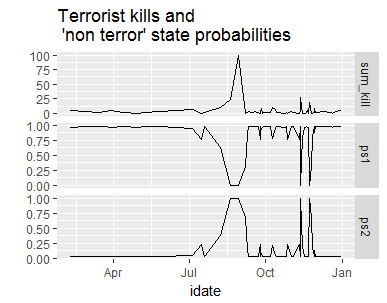
\includegraphics[width=15cm]{Peters_experiment_markdown_files/figure-latex/Rplot02_2003_2004.png}
\caption{Faceted plot of daily death count and probability of emission states due to terrorism from Iraq modelled using a HMM, 2003-2004.}
\label{fig:Rplot02_hmm_2003_2004}
\centering
\end{figure}

\begin{figure}[t]
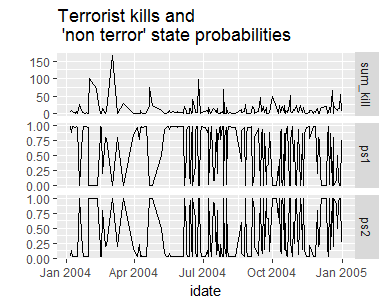
\includegraphics[width=15cm]{Peters_experiment_markdown_files/figure-latex/Rplot02_2004_2005.png}
\caption{Faceted plot of daily death count and probability of emission states due to terrorism from Iraq modelled using a HMM, 2004-2005.}
\label{fig:Rplot02_2004_2005}
\centering
\end{figure}

\begin{figure}[t]
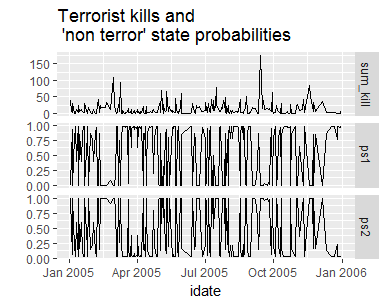
\includegraphics[width=15cm]{Peters_experiment_markdown_files/figure-latex/Rplot02_2005-2006_hmm.png}
\caption{Faceted plot of daily death count and probability of emission states due to terrorism from Iraq modelled using a HMM, 2005-2006.}
\label{fig:Rplot02_2005_2006}
\centering
\end{figure}

\begin{figure}[t]
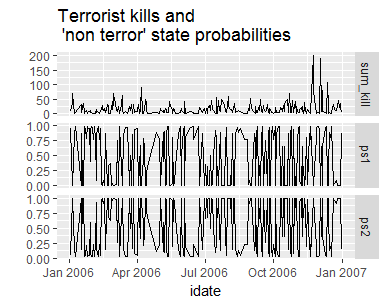
\includegraphics[width=15cm]{Peters_experiment_markdown_files/figure-latex/Rplot02_2006_2007.png}
\caption{Faceted plot of daily death count and probability of emission states due to terrorism from Iraq modelled using a HMM, 2006-2007.}
\label{fig:Rplot02_2006_2007}
\centering
\end{figure}

\begin{figure}[t]
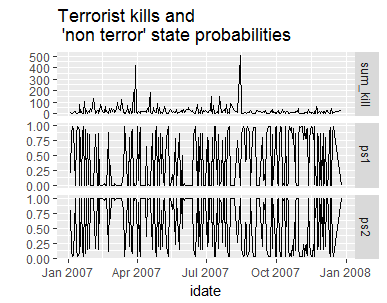
\includegraphics[width=15cm]{Peters_experiment_markdown_files/figure-latex/Rplot02_2007_2008.png}
\caption{Faceted plot of daily death count and probability of emission states due to terrorism from Iraq modelled using a HMM, 2007-2008.}
\label{fig:Rplot02_2007_2008}
\centering
\end{figure}

\begin{figure}[t]
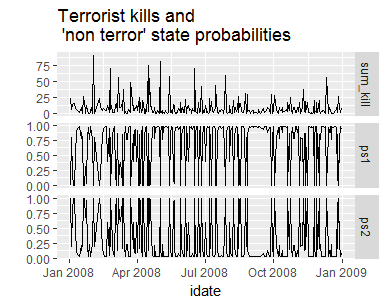
\includegraphics[width=15cm]{Peters_experiment_markdown_files/figure-latex/Rplot02_200_2009.png}
\caption{Faceted plot of daily death count and probability of emission states due to terrorism from Iraq modelled using a HMM, 2008-2009.}
\label{fig:Rplot02_2008_2009}
\centering
\end{figure}

\begin{figure}[t]
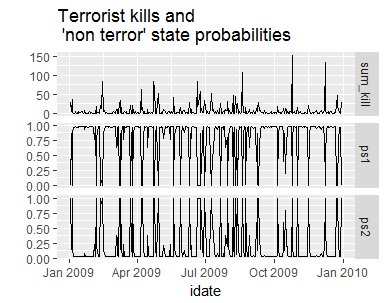
\includegraphics[width=15cm]{Peters_experiment_markdown_files/figure-latex/Rplot02_2009_2010.png}
\caption{Faceted plot of daily death count and probability of emission states due to terrorism from Iraq modelled using a HMM, 2009-2010.}
\label{fig:Rplot02_2009_2010}
\centering
\end{figure}

\begin{figure}[t]
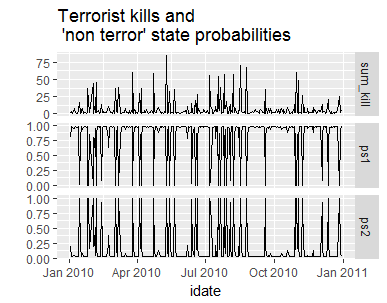
\includegraphics[width=15cm]{Peters_experiment_markdown_files/figure-latex/Rplot02_2010_2011_HMM.png}
\caption{Faceted plot of daily death count and probability of emission states due to terrorism from Iraq modelled using a HMM, 2010-2011.}
\label{fig:Rplot02_2010_2011_HMM}
\centering
\end{figure}

\begin{figure}[t]
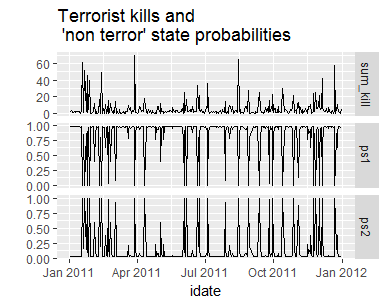
\includegraphics[width=15cm]{Peters_experiment_markdown_files/figure-latex/Rplot02_2011_2012.png}
\caption{Faceted plot of daily death count and probability of emission states due to terrorism from Iraq modelled using a HMM, 2011-2012.}
\label{fig:Rplot02_2011_2012}
\centering
\end{figure}

\begin{figure}[t]
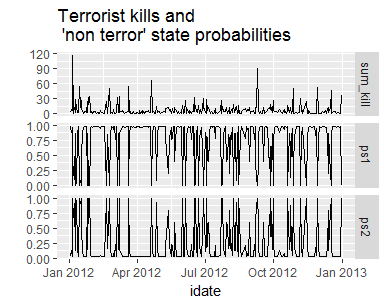
\includegraphics[width=15cm]{Peters_experiment_markdown_files/figure-latex/Rplot02_2012_2013_HMM.png}
\caption{Faceted plot of daily death count and probability of emission states due to terrorism from Iraq modelled using a HMM, 2012-2013.}
\label{fig:Rplot02_2012_2013_HMM}
\centering
\end{figure}

\begin{figure}[t]
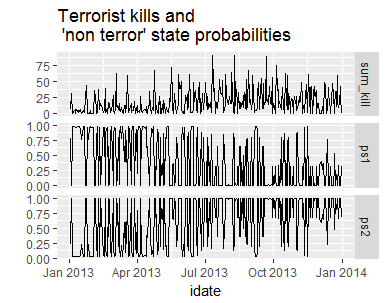
\includegraphics[width=15cm]{Peters_experiment_markdown_files/figure-latex/Rplot02_2013_2014.png}
\caption{Faceted plot of daily death count and probability of emission states due to terrorism from Iraq modelled using a HMM, 2013-2014.}
\label{fig:Rplot02_2013_2014_HMM}
\centering
\end{figure}

\section{Discussion}

The aim of this appendix which was a preliminary examination of the data was two fold:
\begin{itemize}
\item Firstly to gain a understanding of underlying trends in the data and the relationships between the different data dimensions.
\item Secondly to ascertain which modelling techniques may be appropriate to the data and which would need further consideration.
\end{itemize}
A mix of descriptive data visualizations, regio and regio temporal visualizations, dimension reduction and the resulting visualization of the dimensions. Preliminary modelling of count of deaths due to terrorism (country specific to Iraq) was carried out.
Time series plots of Descriptive visualizations of temporal relationships between different weapon, attack vector and regions were carried out using stacked bar charts, this allowed visual encodings  of 3 data dimensions. From the resulting data visualization it was clear to see the resulting regio-temporal relationships and  attack and weapon type relationships. A clear regio-specific trend can be seen, where Western Europe was the predominant region in the 1970's, Central America and South America in the 1980's, Africa in the 1990's and the 2000's dominated by South Asia and the Middle East. 

This view was supplemented by creating a faceted regio-temporal sums of deaths due to terrorism by decade and the individual countries which are the foremost countries and are easy to distinguish. There is also a clear relationship between weapon type vector(the foremost attack vectors being armed assault) and attack type (bombings and explosions). 

The understanding gained via the various visualization techniques described previously was further enhanced using dimension reduction techniques (CA and MCA) and interactions between multiple categorical variables were evaluated. Specifically certain associations can be seen that are not discernible from the descriptive data visualizations. The dimension reduction techniques when used with interactive visualization techniques based upon the D3 framework made this possible as it allowed analysis to be focussed very deeply onto the data and uncover underlying associations between the different levels of the categorical data being examined. The interactive visualization packages plotly package proved adept at this. Using these techniques it was possible to ascertain particularly relationships between attack types and weapons, specifically chemical weapons and unarmed assaults. 

2009 and attacks against the police while 2003 was strongly associated with attacks against governments. These techniques were useful at showing a change in behaviour in terrorism but did not give any particular insight into uncovering a change in intensity in terrorism.

Cluster analysis was also carried out on terrorist incidents in Iraq and Syria and the incidents (using both kernel density estimation and k-means clustering) appeared to be largely clustered in urban areas. Iraq and Syria were chosen as the descriptive visualization had shown these countries along with Afghanistan to be predominant in terms of terrorist activity. Cluster analysis (and kernel density estimation) was able to identify (by overlaying the the clusters of the incidents on an interactive map) a rural-urban divide in terms of where incidents occur. This method suffered from a number of problems, as an unsupervised method, the number of clusters must be empirically derived so its country wide application to look for a global trend of rural urban divide in terms of where terrorist incidents occur would be difficult to do as the optimal k value would have to be ascertained per country. Kernel density estimation used to create thematic maps showed similar information to the spatial clustering, and again illustrated that attacks in Iraq and Syria were largely concentrated in urban areas.

After carrying out the descriptive statistical visualizations, cluster analysis and dimension reduction techniques a number of preliminary modelling techniques were applied to countries in specific regions based on their pre-eminence in terms of terrorism activity (both death count and incident count). These techniques and the choice of preliminary  modelling technique used and their use case was informed by the literature review of current research into terrorism research using electronic event databases concerning terrorism. 

Either using terrorist data to predict or forecast future trends in incidents or else the use of the GTD to help explain the effects of specific strategies. The aim of the preliminary studies was also to see how universal the application of a technique would be and what reach it would have (could it identify changes in intensity in terrorism and the factors causing them?), how easy would the technique be to apply across multiple regions? Another aim of the analysis was to challenge (by confirming or denying) existing conceptions held about terrorism.

Examples of such conceptions would be what was the effect of the US surge in Iraq and what, if any were the underlying reasons for ISIS's rapid rise, was it a inaction by the West?, what were the effects of the interventions of the coalition forces  or could the GTD even answer this question. What were the limitations of the data or the type of data held in the GTD and how easy it to augment the GTD with other data sources?

Preliminary modelling of count data was done with both regression (and alternative methodologies) analysis on Iraq's counts of deaths due to terrorism to explain the counts of deaths and the interdependencies with particular US, Iraqi or insurgent actions along with the months (since 1970, when records of terrorism began in the PGIS, the precusors of the GTD). 

HMM's were used to carry out a preliminary time series analysis of counts of deaths due to terrorism In Iraq. From the analysis of the emitted state probabilities and the frequency of the states it is possible to see particular epoch and a change of epochs from one of relatively low levels of terrorism to another of a high levels of terrorism. The aim of the modelling was to evaluate how effective the modelling tool. Both modelling count data using regression and using HMM's proved problematic. 

When modelling count data, the count regression models were found to suffer from issues with them being not specified correctly or else assumptions regarding the modelling technique being violated.  When using Poisson regression (and its related techniques of quasi-Poisson and negative binomial regression) to model the count data, the models were found to suffer from being either over dispersed or having a poor goodness of fit. Transformations can be particularly useful when trying to increase the ability of a particular modelling technique to be able to fit to the data 
before applying simple multivariate linear regression or by steadying variance. However log transforms does suffer from a number of known shortcomings, including its inability to deal with zero observations requiring the addition of one to a value before it is log transformed and these methods have performed poorly in the past when compared to using models established using Poisson, Quasi-Poisson or negative binomial distributions \citep{o2010not}. Ascertaining which model performed best though also proved difficult as different 'goodness of measurements' are used across lm's and glm's. 

While HMM's proved useful at identifying different epochs (an epoch of high numbers of deaths due to terrorism, or an epoch of low deaths due to terrorism) of terrorist activity and the onset of these epochs, it did suffer from problems of generalizability and understandability. Such a model would have undoubted usefulness from a number of standpoints, such a model would be capable of informing risk management and insurance decisions (from an insurance underwriting perspective) or from a governmental point of view identifying when to deploy or mobilise armed forces. However these models due to their unsupervised nature would also prove problematic to deploy globally on a country wide basis as much like clustering the number of transition states would have to be empirically derived. However models that would be able to ascertain similar changes in epoch or outbreaks in terrorist activity would be useful in serving as an early warning system or alarm system to analysts in modelling terrorism. The problems of understandability is due to the output being difficult to understand for non statistically trained analyst as the output which is a transition state probability is difficult to understand. This problem can be addressed by turning the transition probability to a class if it exceeds a probability threshold (this is commonly set to 50\% in machine learning, but could be tuned), if this threshold is exceed the specific period is defined as belonging to a particular class. The facet class /count deaths plots are shown in figure and \ref{fig:Rplot02_2006_facstate_HMM},\ref{fig:Rplot02_2007_facstate_HMM} and \ref{fig:Rplot02_2008_facstate_HMM}. It is quite clear from these epoch plots the effect of the 2007 surge. In 2006  for a large part of the year the predominant epoch is one of being in a 'terror state' (encoded as state 1 the blue coloured points). 

In 2007 for a large part of the year the predominant epoch is one of being in a 'terror state'. While in 2008 the opposite is true with the predominant epoch being one of a 'non terror state' (encoded as state 0 the red coloured points), which would give some support for the  surge having a positive effect and infact reducing terrorism as the post surge period is correlated with a reduction in number of days being in an epoch of a 'terror state'.

\begin{figure}[t]
\includegraphics[width=15cm]{Peters_experiment_markdown_files/figure-latex/Capture_HMM_2006state_kills.png}
\caption{Faceted plot of daily death count and epoch classification due to terrorism from Iraq modelled using a HMM, 2006.}
\label{fig:Rplot02_2006_facstate_HMM}
\centering
\end{figure}


\begin{figure}[t]
\includegraphics[width=15cm]{Peters_experiment_markdown_files/figure-latex/Capture_HMM_2007state_kills.png}
\caption{Faceted plot of daily death count and epoch classification due to terrorism from Iraq modelled using a HMM, 2007.}
\label{fig:Rplot02_2007_facstate_HMM}
\centering
\end{figure}

\begin{figure}[t]
\includegraphics[width=15cm]{Peters_experiment_markdown_files/figure-latex/Capture_HMM_2008state_kills.png}
\caption{Faceted plot of daily death count and epoch classification due to terrorism from Iraq modelled using a HMM, 2008.}
\label{fig:Rplot02_2008_facstate_HMM}
\centering
\end{figure}

Understanding of the effects of US troop surge in 2007 can be further enhanced by aggregating up the terror epoch days (per month) (see figure~\ref{fig:Rplot02_2008_facstate_HMM_agg}) and the deaths per month and creating a faceted plot of both of these with the daily death count plot for the period 2006-2009. It is clear from the plot that the monthly number of 'terror epoch days' was higher pre surge compared to post surge and the surge did see an initial increase in 'terror epoch days'. This again would give some support to the notion that the troop surge did have a positive effect on reducing terrorism in post invasion Iraq.

\begin{figure}[t]
\includegraphics[width=15cm]{Peters_experiment_markdown_files/figure-latex/Capture_HMM_2006_2009_state_kills_agg.png}
\caption{Faceted aggregate plot of monthly death count and epoch classification due to terrorism from Iraq modelled using a HMM with the daily death count for the same period, 2008.}
\label{fig:Rplot02_2008_facstate_HMM_agg}
\centering
\end{figure}


\section{Conclusion}
This section/appendix focussed on carrying out an exploratory analysis. The reason for this was twofold, to gain an initial understanding of the data and also to gain an understanding of what methods maybe appropriate to analyse the data. To this end, a number of data visualization techniques were used to explore the data along with a combination of data visualization techniques and unsupervised machine learning techniques were used to gain an insight into the data. To analyse time series of count of incidents, time series plots were appropriate to visualize the data using a number of different time intervals (year, month). The time series plots revealed that the intensity of terrorism (in terms of counts of terrorism and counts of deaths due to terrorism) was increasing. Since records began to be recorded in the 1970’s terrorism has been on the increase, though in the 1990’s the trajectory appeared to slow down or level off. In the 2000’s post September 11th 2001, again (the counts of deaths due to terrorism) increased followed by a much more pronounced increase post the US invasion of Iraq. The emergence of ISIS (2012) has also seen a large increase in the intensity of terrorism. 

By stratifying the time series by region and plotting the time series plot, a regio-temporal relationship is also apparent. That is, before the 1980’s no one region is seen to be dominant in terms of terrorism, while in the 1980’s central America and South America is the dominant region. Again in the 1990’s no particular no one region appears to be dominant though, South Asia, South America , Middle East and North Africa and Sub-Saharan Africa appear to be the prevalent regions. In the 2000’s and 2010’s  the Middle East and North Africa, Sub-Saharan Africa and South Asia are the predominant areas.  By utilizing a stacked choropleths (a thematic map of deaths due to terrorism) by decade, an enhanced understanding of the regional time-series plots could be attained. 

One can see from the choropleth that in the 1970’s terrorism appears to be dominated by the United Kingdom and Iran. The 1980’s  by Central and South American countries, particularly Columbia, El Salvador, Nicaragua and Peru and India. During the 1990’s the pattern becomes more diffuse with terrorism being dominant across a number of countries Algeria, South Africa, India and Turkey. Russia also starts to become prevalent in the 1990’s in terms of deaths due to terrorism and this trend continues into the 2000’s. The 2000’s sees terrorism almost disappear from countries were it was previously prevalent in South America (Colombia and Peru). South Asia (Afghanistan, Pakistan and India) and Iraq (terrorism only starts to increase after the US led invasion of Iraq). In the 2010’s terrorism becomes dominated by the Middle East (Iraq and Syria), South Asia (Afghanistan and Pakistan) and Nigeria. The use of stacked choropleths proved particularly at showing the regio-temporal shift in terrorism over the decades though is limited by the number of epochs that the stacked choropleth can accommodate. If too many epochs are used the display of the information becomes difficult, as one can only (even with the use of interactive graphics) process a limited number of stacked choropleths. While using too few epochs the visualization suffers from lack of detail and no patterns become discernible. The use of analysis libraries (the r googleVis library) allowed the creation of very rich data visualizations, free of charge that offer a large amount of insight into spatio-temporal patterns of terrorism.

Stacked barplots also proved useful at exploring how changes in attack vector or weapon type changed with time. It is quite clear to see that since the 1970’s armed assault and bombings become the prevalent attack types. While since the 1970’s explosives/bombs/dynamite has emerged as the dominant weapon type.  While this data visualization methodology proved useful it was limited to the number of dimensions that could be visualized. To overcome this, a number of unsupervised techniques used in conjunction with interactive data visualization techniques were used. 

Correspondence analysis, particularly multiple correspondence analysis were used to understand interactions and associations between multiple data dimensions. The use of interactive data visualizations in tandem with MCA through the use of interactive bi-plots allowed associations between different categorical levels to be made. Bi-plots are a type of scatterplot which allows data on both the transformed dimensions,  original variables and samples to be displayed together. By displaying the output in an interactive form if the visualization becomes too dense the analyst can either zoom in a particular are of interest or else can temporarily remove particular variables to allow a clearer understanding of the association between variables. From the use of MCA a number of associations could be observed these were:

\begin{itemize}
\item There is a vigorous association between the year 1974 and terrorist attacks on non state militia or terrorists.
\item Unarmed assaults are largely associated with chemical weapons use.
\item The year 2003 is strongly associated with attacks against government, while the year 2009 shows a strong association between attacks targeting police.  
\item The year 1994 is strongly associated with attacks using weapon types sabotage equipment and mellee weapons against facilities and infrastructure.
\end{itemize}

These methods allowed uncovering of interactions or associations that be difficult to detect by other methods but their use with the GTD did pose some problems. Particularly trying to analyse the associations between terrorist groups with particular epochs was difficult due to the large number of groups or more apt the numerous designations for groups. 

Geo-spatial analysis was another exploratory analysis method that was possible by combining either clustering or kernel density estimation.  Such techniques in conjunction with interactive data visualizations allow an analyst to determine centres of activity for terrorism or the spatial dispersion of incidents whether they are occurring in rural or urban areas. 

Spatial K-means clustering of terrorist events showed large concentrations of terrorist incidents in mostly urban areas,specifically around the Sunni triangle and Alepo (Syria). 

The preliminary modelling consisted of two distinct parts Regression modelling of count of deaths due to terrorism in Iraq and time series count modelling using HMM’s.

Preliminary modelling was carried out on the GTD and an enhanced dataset sourced from the GTD. The enhanced dataset was created by appending data sourced on Iraqi and US presidential terms and US troop activity regarding the invasion along with information regarding periods of major insurgency activity within Iraq. US troop activity would be concerned with major actions by Allied and US forces concerning the invasion of Iraq , the 2007 surge to combat the Iraqi insurgency and the subsequent drawdown and eventual pull out and with-drawl of Allied and US troops. While count models were used they proved to be problematic and suffered from being incorrectly specified.   

HMM’s were also used to model the count data using two different states (one representing a state of ‘high level terrorism’ and the other one of ‘low level terrorism’). While this model worked well at being able to classify a certain period of time being in one of the above epoch’s it proved difficult to generalize and would be of limited use in modelling count terrorism data. For this reason alternative methodologies were employed in the modelling chapter (chapter 5).

